% !TEX root = ../IPLeiriaMain.tex

\section{Introduction}

L'application a été développée selon une architecture MVC (Modèle-Vue-Contrôleur), afin d'assurer une séparation claire des préoccupations, une évolutivité et une facilité de maintenance. Cette approche permet de structurer l'application en trois couches distinctes qui communiquent entre elles de manière organisée, offrant ainsi une plus grande flexibilité dans le développement et la maintenance.

Le choix des technologies a été guidé par la volonté de combiner performance, fiabilité et simplicité d’utilisation, aussi bien pour les développeurs que pour les utilisateurs finaux.

\section{Environnement de développement et gestion du projet}

Pour garantir un travail efficace et collaboratif, plusieurs outils ont été mobilisés :

\begin{itemize}
    \item \textbf{Visual Studio Code :} utilisé pour le développement du Front-End Angular.
    \item \textbf{IntelliJ IDEA :} choisi pour le développement du Back-End Spring Boot.
    \item \textbf{ECS Projects :} outil interne de gestion de projet, basé sur un système de tickets créés par le manager, suivis jusqu’à leur validation.
    \item \textbf{GitLab :} plateforme de gestion de versions, assurant la centralisation du code, la création de branches et la collaboration entre les développeurs.
\end{itemize}

\section{Architecture MVC}

L'architecture mise en place repose sur le pattern Modèle-Vue-Contrôleur (MVC) avec une séparation claire entre les différentes couches de l'application :

\begin{itemize}
    \item \textbf{Modèle (Model) :} Gère les données et la logique métier. Dans le projet, il est responsable de l'interaction avec la base de données et de la gestion des données des projets, utilisateurs et soumissions.
    \item \textbf{Vue (View) :} Représente la couche de présentation, c'est-à-dire ce que l'utilisateur voit à l'écran. Elle utilise HTML et CSS pour afficher les données fournies par le modèle.
    \item \textbf{Contrôleur (Controller) :} Fait le lien entre le modèle et la vue. Il traite les entrées utilisateur, effectue les opérations sur le modèle et met à jour la vue en conséquence.
\end{itemize}

% --- IMAGE ---
\begin{figure}[H]
    \centering
    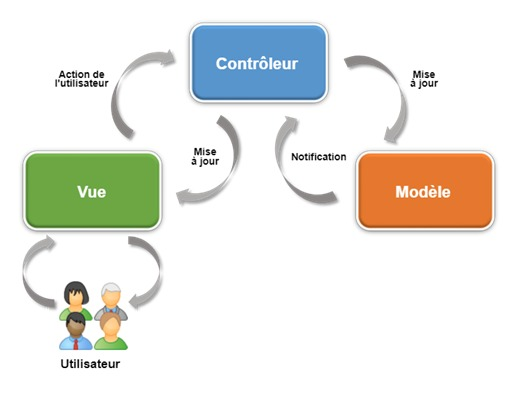
\includegraphics[width=0.9\textwidth]{Figures/Illustration_modele_mvc.jpg}
    \caption{Illustration modèle MVC}
    \label{fig:mvc-architecture}
\end{figure}

Cette organisation permet de maintenir une séparation claire des préoccupations, facilitant ainsi le développement, la maintenance et l'évolution de l'application.

\section{Technologies utilisées}

\begin{itemize}
    \item \textbf{Back-End : Spring Boot (Contrôleur et Modèle)}
    \begin{itemize}
        \item Implémentation des contrôleurs REST pour la gestion des requêtes.
        \item Développement des entités JPA et repositories pour la couche modèle.
        \item Services métier pour la logique applicative.
        \item Gestion de la sécurité et des règles métier.
    \end{itemize}

    \item \textbf{Front-End : Angular (Vue)}
    \begin{itemize}
        \item Création d'une interface dynamique et réactive.
        \item Gestion des routes et des composants.
        \item Interaction avec le Back-End via HTTP.
        \item Présentation des données utilisateur.
    \end{itemize}

    \item \textbf{Base de données : MySQL}
    \begin{itemize}
        \item Stockage structuré et fiable des données.
        \item Intégration avec Spring Data JPA pour les opérations de persistance.
        \item Relations entre entités pour la cohérence des données.
    \end{itemize}

    \item \textbf{Node.js \& NPM}
    \begin{itemize}
        \item Nécessaires au fonctionnement d'Angular et à la gestion des dépendances.
    \end{itemize}
\end{itemize}

%======================================================================
%    SECTION INTERFACES (VERSION FINALE)
%======================================================================

\section{Présentation des interfaces}

Les interfaces développées dans le cadre de ce projet sont conçues pour assurer une gestion efficace et centralisée de la plateforme de gestion de projets. Chaque interface répond à un besoin métier précis, qu'il s'agisse de la gestion des projets, du suivi des tâches, de la planification des sprints ou de la configuration des paramètres système.

L'ergonomie et la fluidité d'utilisation ont été au centre de la conception. Grâce à une structure claire et une navigation intuitive, l'utilisateur peut accéder facilement aux différentes fonctionnalités, garantissant une expérience cohérente et une gestion organisée des activités.

\subsection{Interfaces communes entre les utilisateurs}

% --- Interface Login ---
\begin{figure}[H]
    \centering
    
\includegraphics[width=0.8\textwidth]{Figures/pm screenshots/login.png}
    \caption{Page de connexion de la plateforme MomenTask}
    \label{fig:login}
\end{figure}

Cette interface de connexion présente une page d'accueil moderne avec un design en deux colonnes. La colonne de gauche affiche le logo et la marque "MomenTask" avec le slogan "Effortless momentum for your projects", tandis que la colonne de droite contient le formulaire de connexion. L'interface propose plusieurs options d'authentification : connexion par email/mot de passe, connexion avec Microsoft, et un accès pour les clients potentiels.

% --- Interface Profile ---
\begin{figure}[H]
    \centering
    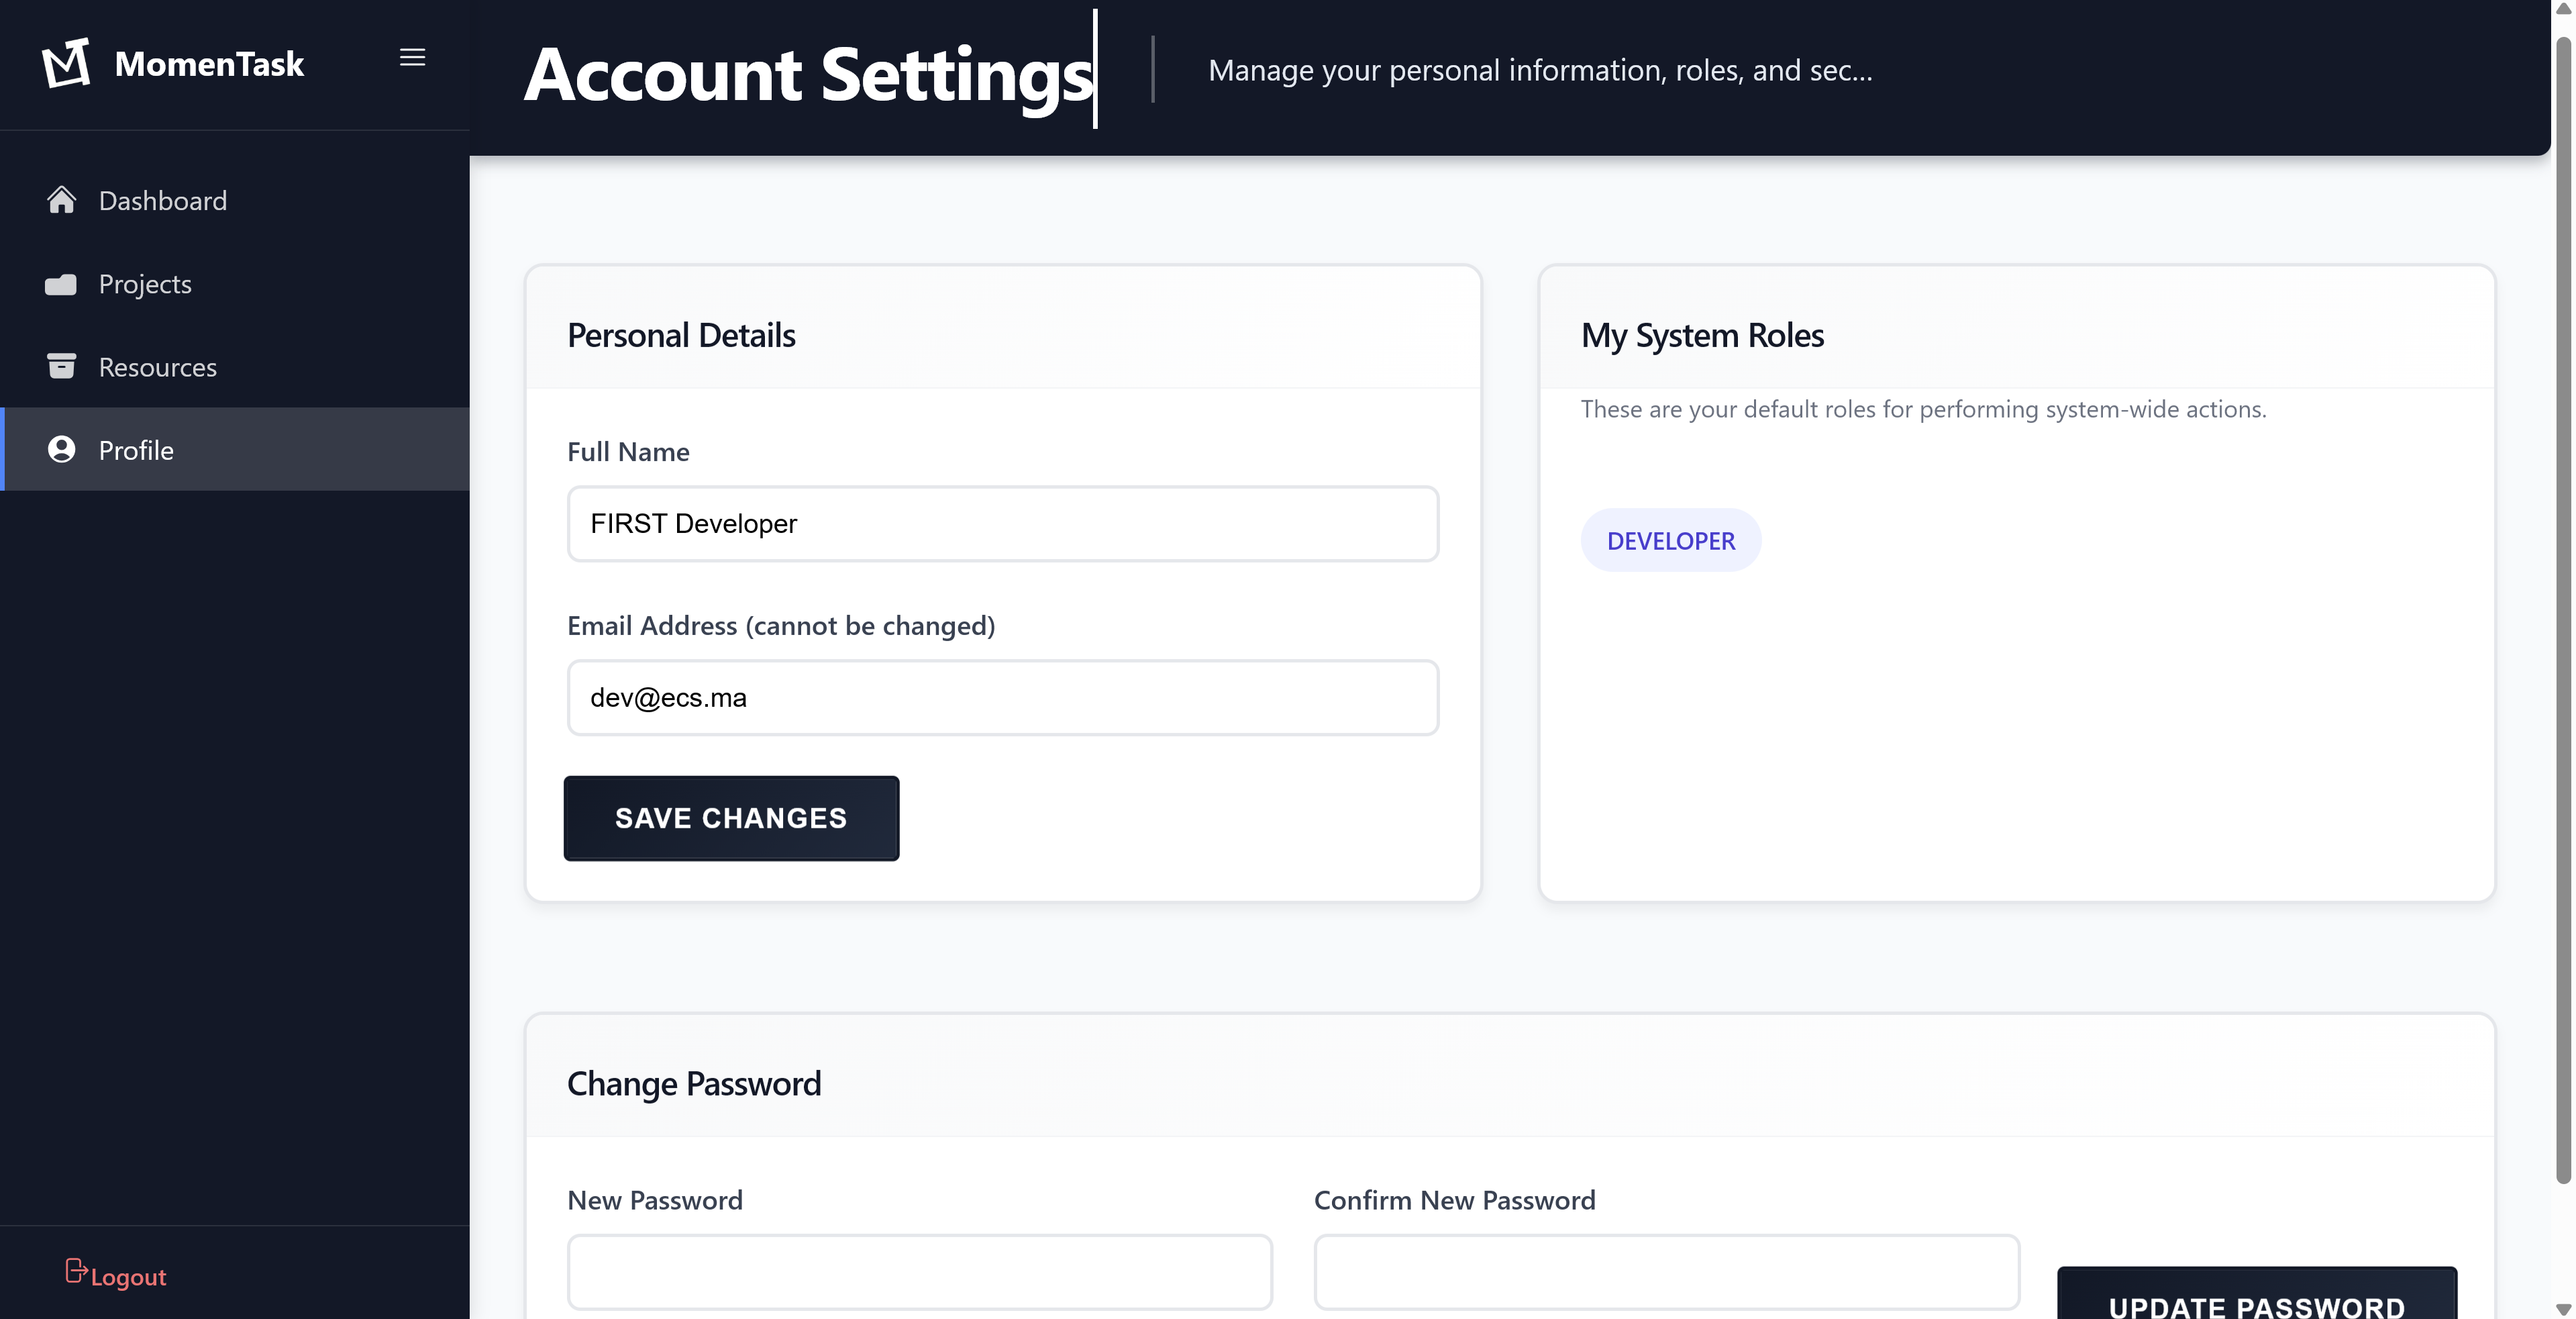
\includegraphics[width=\textwidth]{Figures/pm screenshots/profile.png}
    \caption{Interface de gestion du profil utilisateur}
    \label{fig:profile}
\end{figure}

L'interface de profil permet aux utilisateurs de gérer leurs informations personnelles et leurs paramètres de compte. Elle comprend des sections pour les détails personnels (nom complet, email), les rôles système assignés, et la modification du mot de passe. L'interface affiche clairement le rôle "DEVELOPER" de l'utilisateur connecté et propose des options de mise à jour sécurisées.

% --- Interface Projects List ---
\begin{figure}[H]
    \centering
    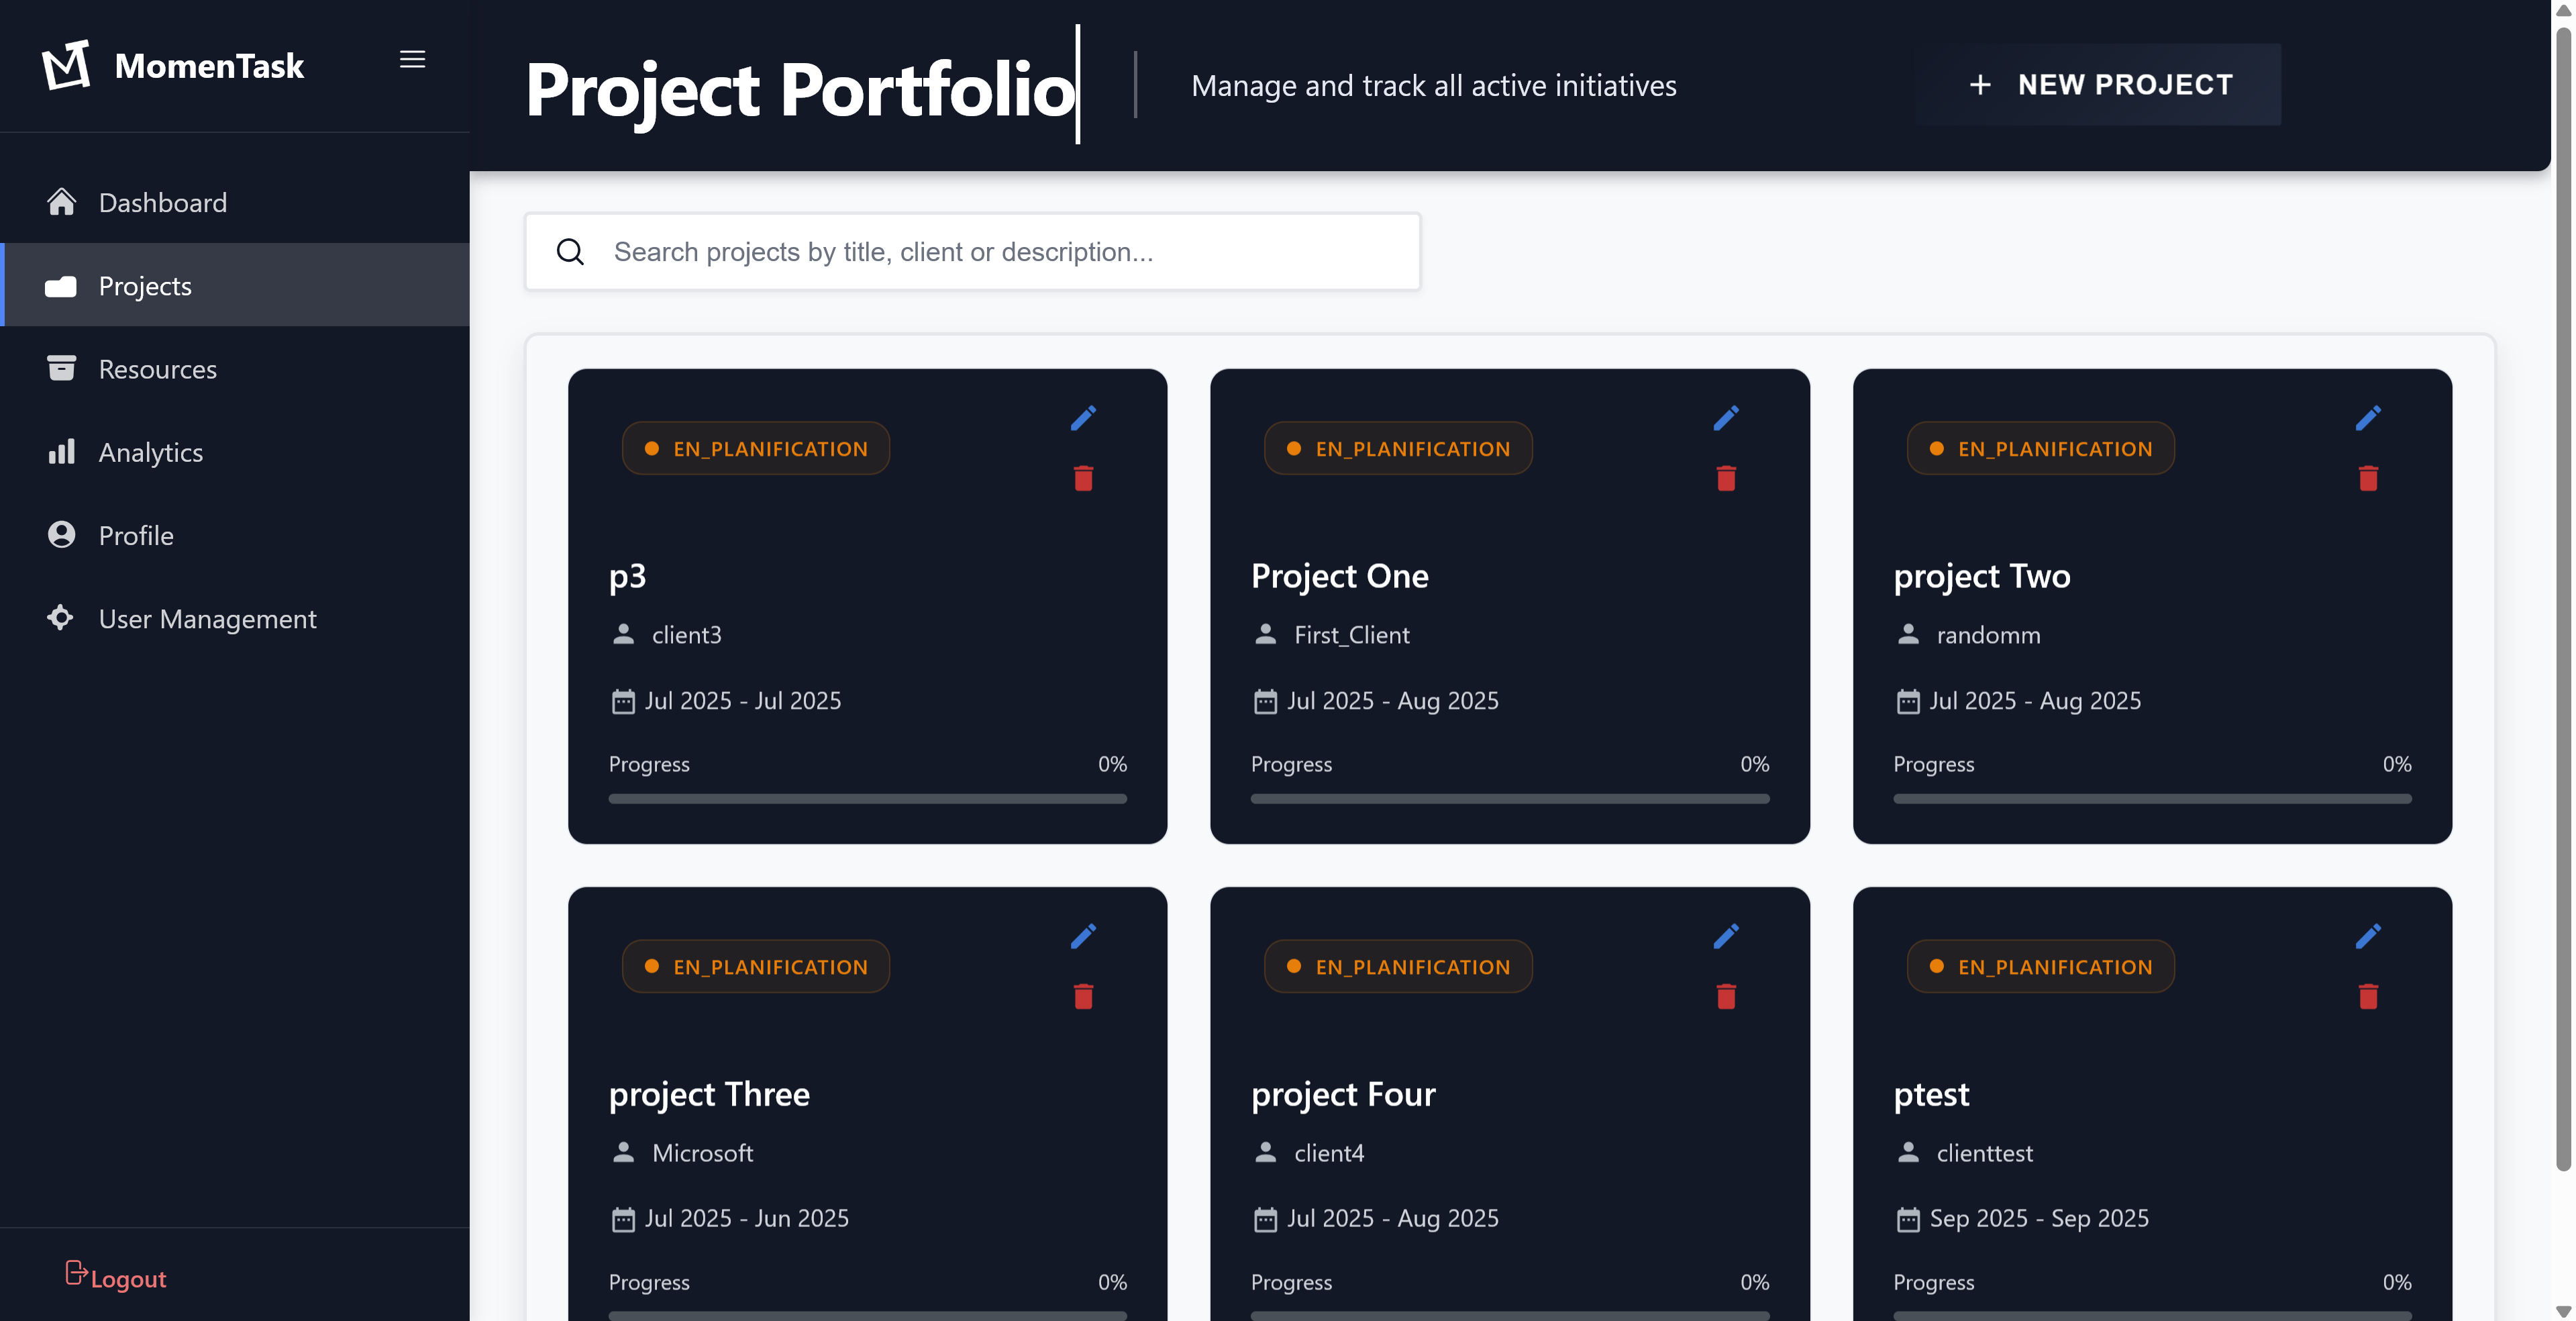
\includegraphics[width=\textwidth]{Figures/pm screenshots/projects list.png}
    \caption{Portefeuille de projets avec vue d'ensemble des initiatives actives}
    \label{fig:projects-list}
\end{figure}

Cette interface présente le portefeuille de projets de l'organisation. Elle affiche une grille de cartes de projets avec des informations clés : statut (EN\_PLANIFICATION), nom du client, dates de début et fin, et barre de progression. Chaque carte propose des actions d'édition et de suppression. La barre de recherche permet de filtrer les projets par titre, client ou description.

\subsection{Vue Client}

% --- Interface Client Form 1 ---
\begin{figure}[H]
    \centering
    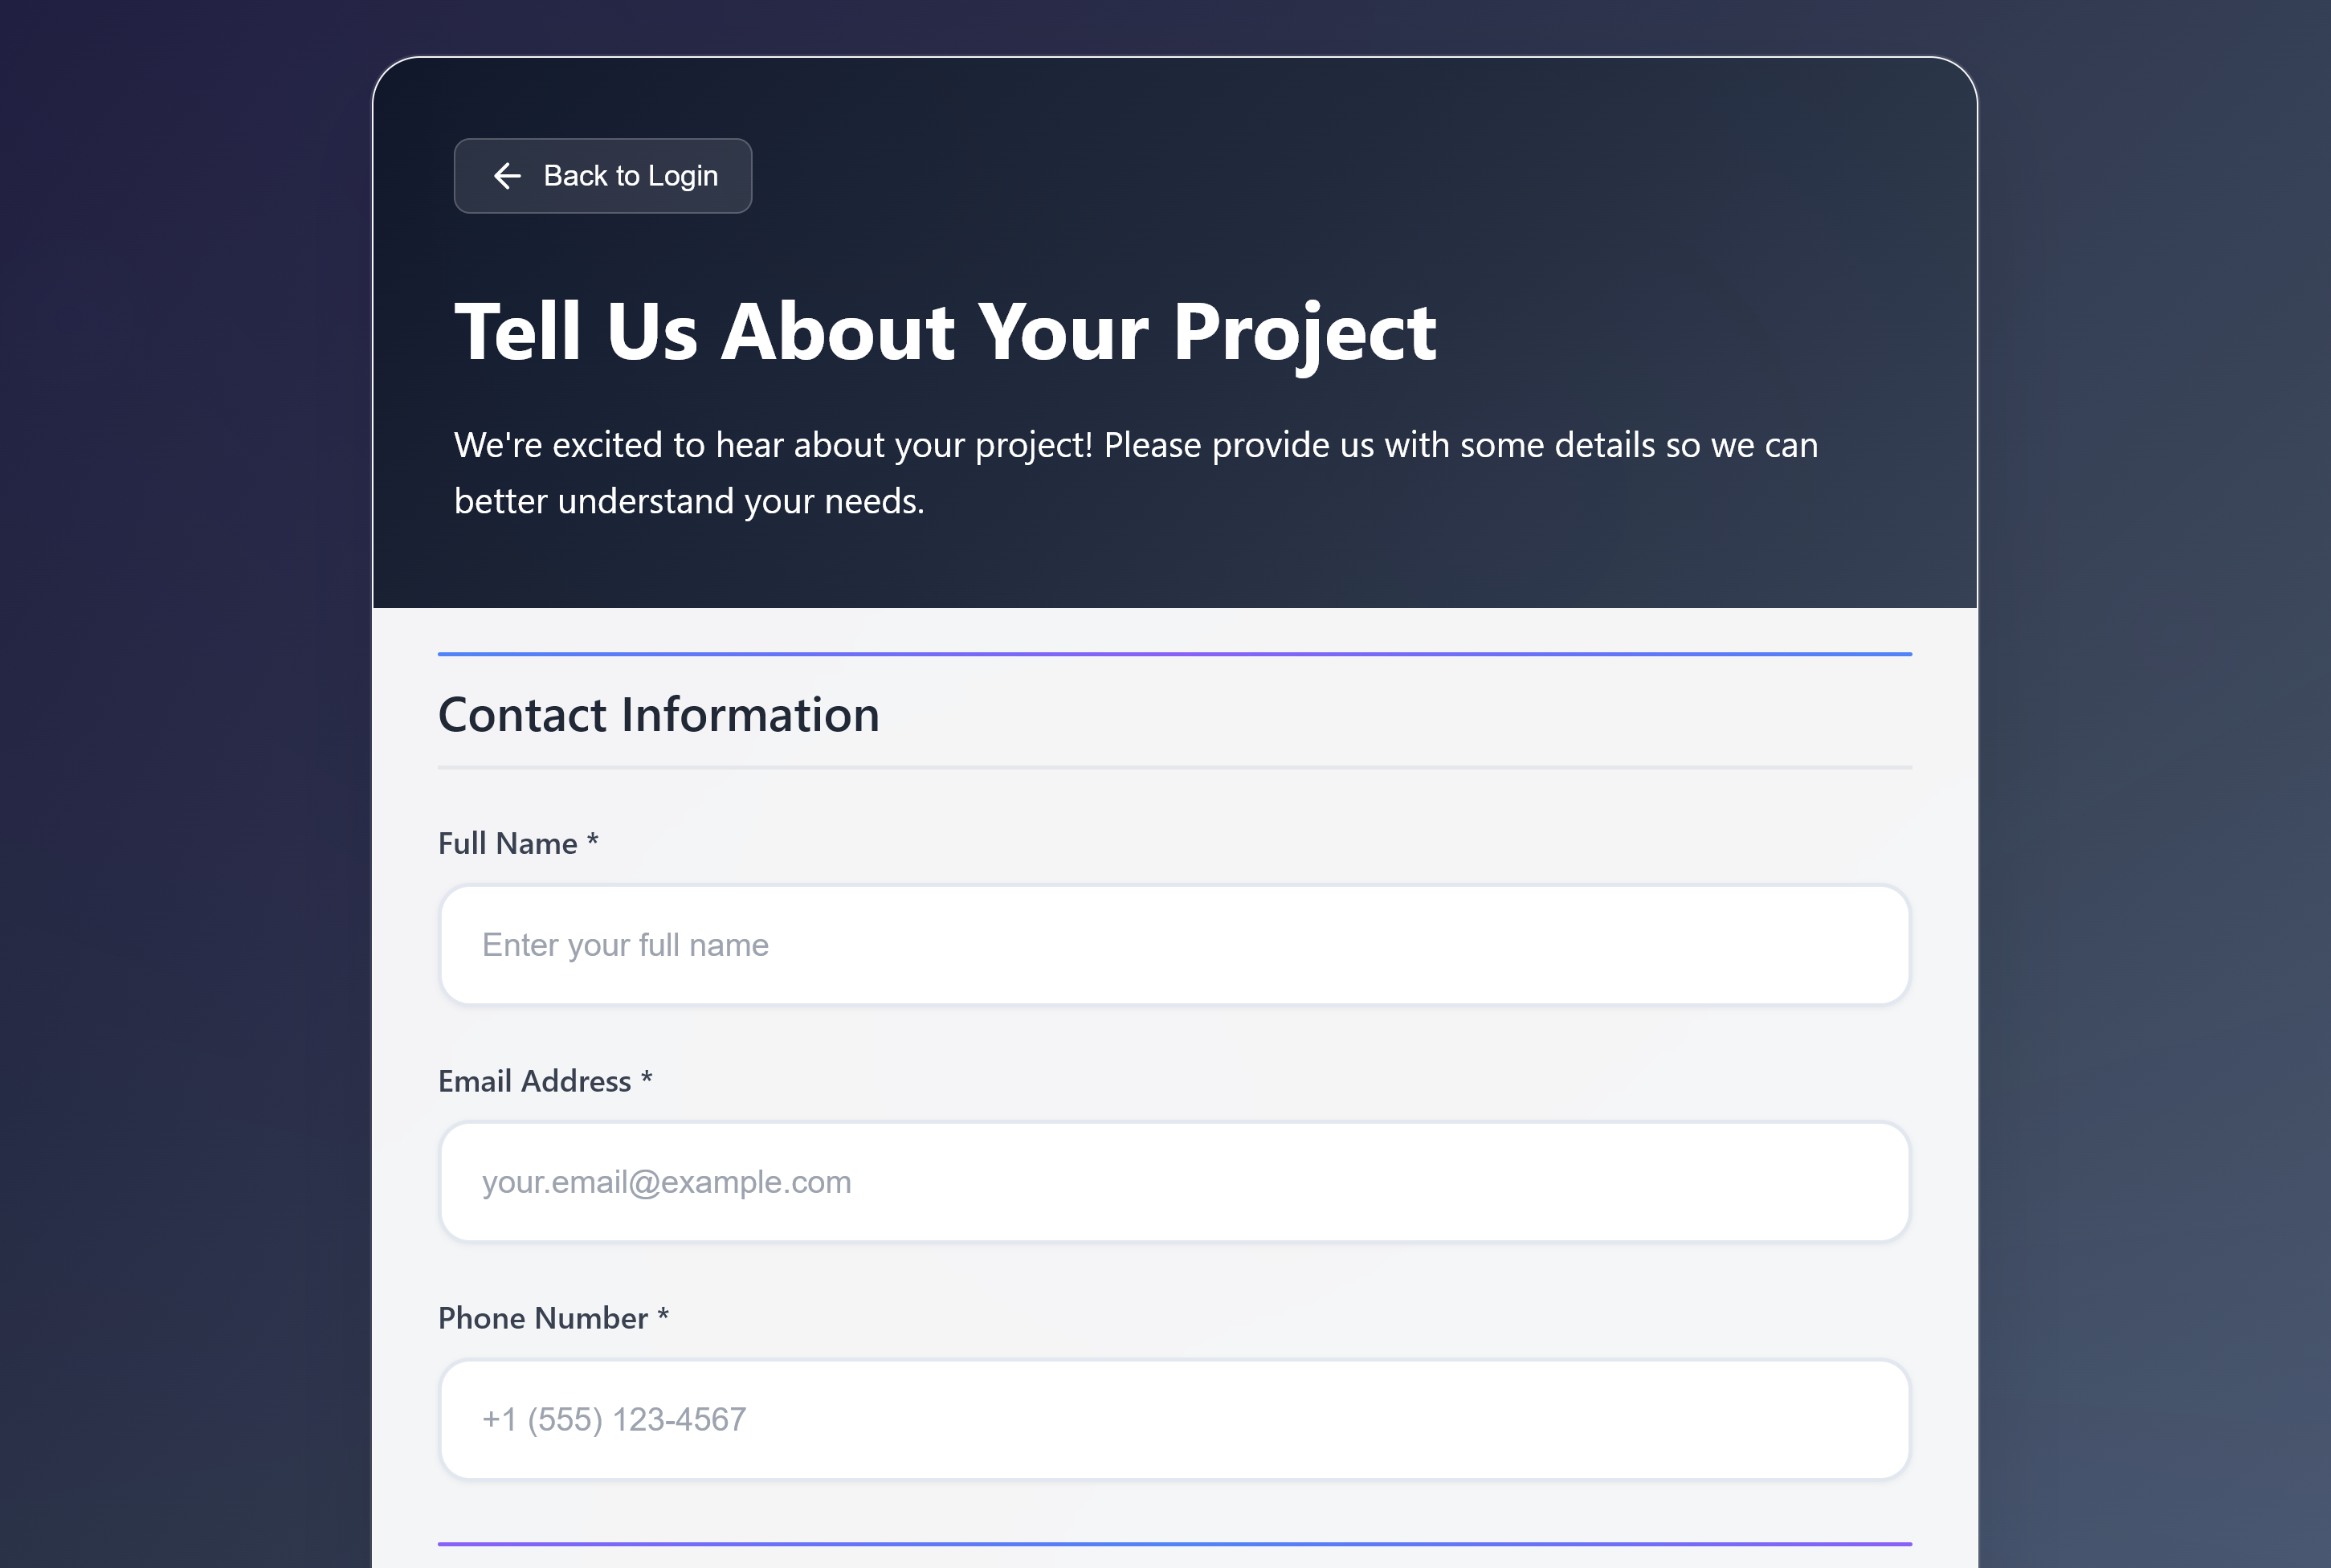
\includegraphics[width=\textwidth]{Figures/pm screenshots/client (not a real user btw)/FORM1.png}
    \caption{Formulaire de demande de projet - Informations de contact}
    \label{fig:client-form1}
\end{figure}

Cette interface permet aux clients potentiels de soumettre leurs demandes de projet. Le formulaire commence par la collecte des informations de contact essentielles : nom complet, adresse email et numéro de téléphone. L'interface est conçue pour être intuitive et accessible, avec des champs obligatoires clairement marqués et des placeholders informatifs.

% --- Interface Client Form 2 ---
\begin{figure}[H]
    \centering
    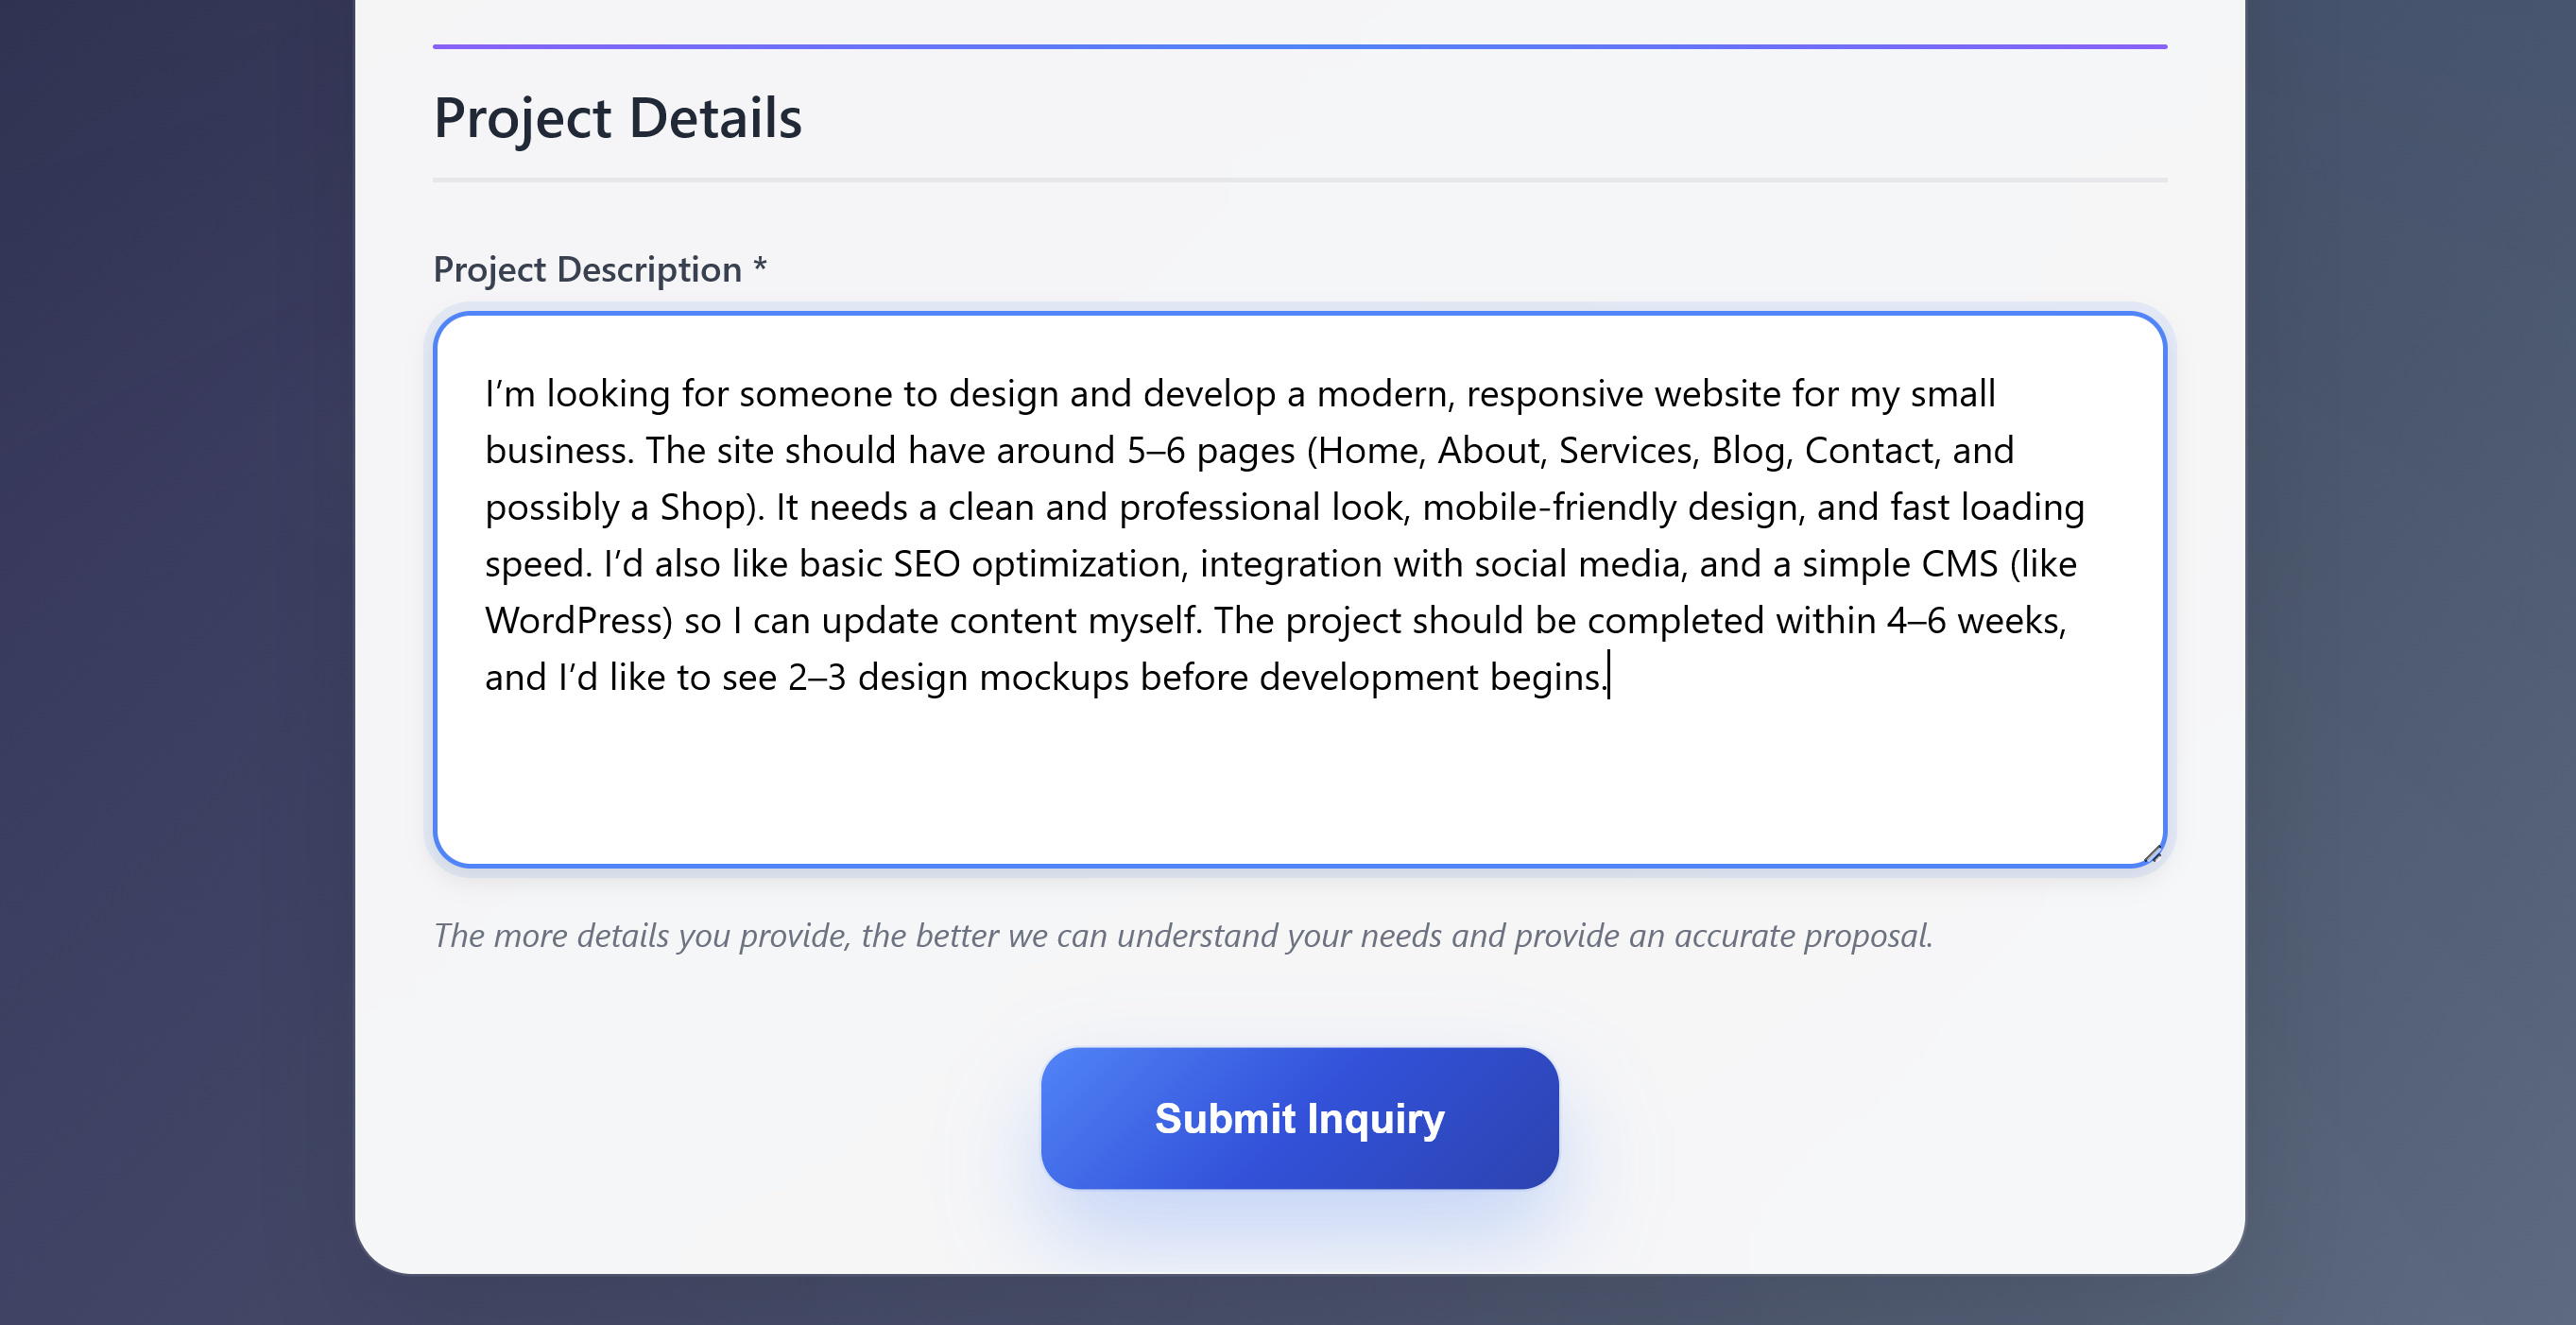
\includegraphics[width=\textwidth]{Figures/pm screenshots/client (not a real user btw)/FORMPART2.png}
    \caption{Formulaire de demande de projet - Description détaillée}
    \label{fig:client-form2}
\end{figure}

La deuxième partie du formulaire client se concentre sur la description détaillée du projet. Cette interface présente un champ de texte étendu où le client peut décrire ses besoins spécifiques, ses objectifs, et ses contraintes. L'exemple montre une demande de développement de site web avec des spécifications précises concernant les pages, le design, l'optimisation SEO, et les délais de livraison.

% --- Interface Client Confirmation ---
\begin{figure}[H]
    \centering
    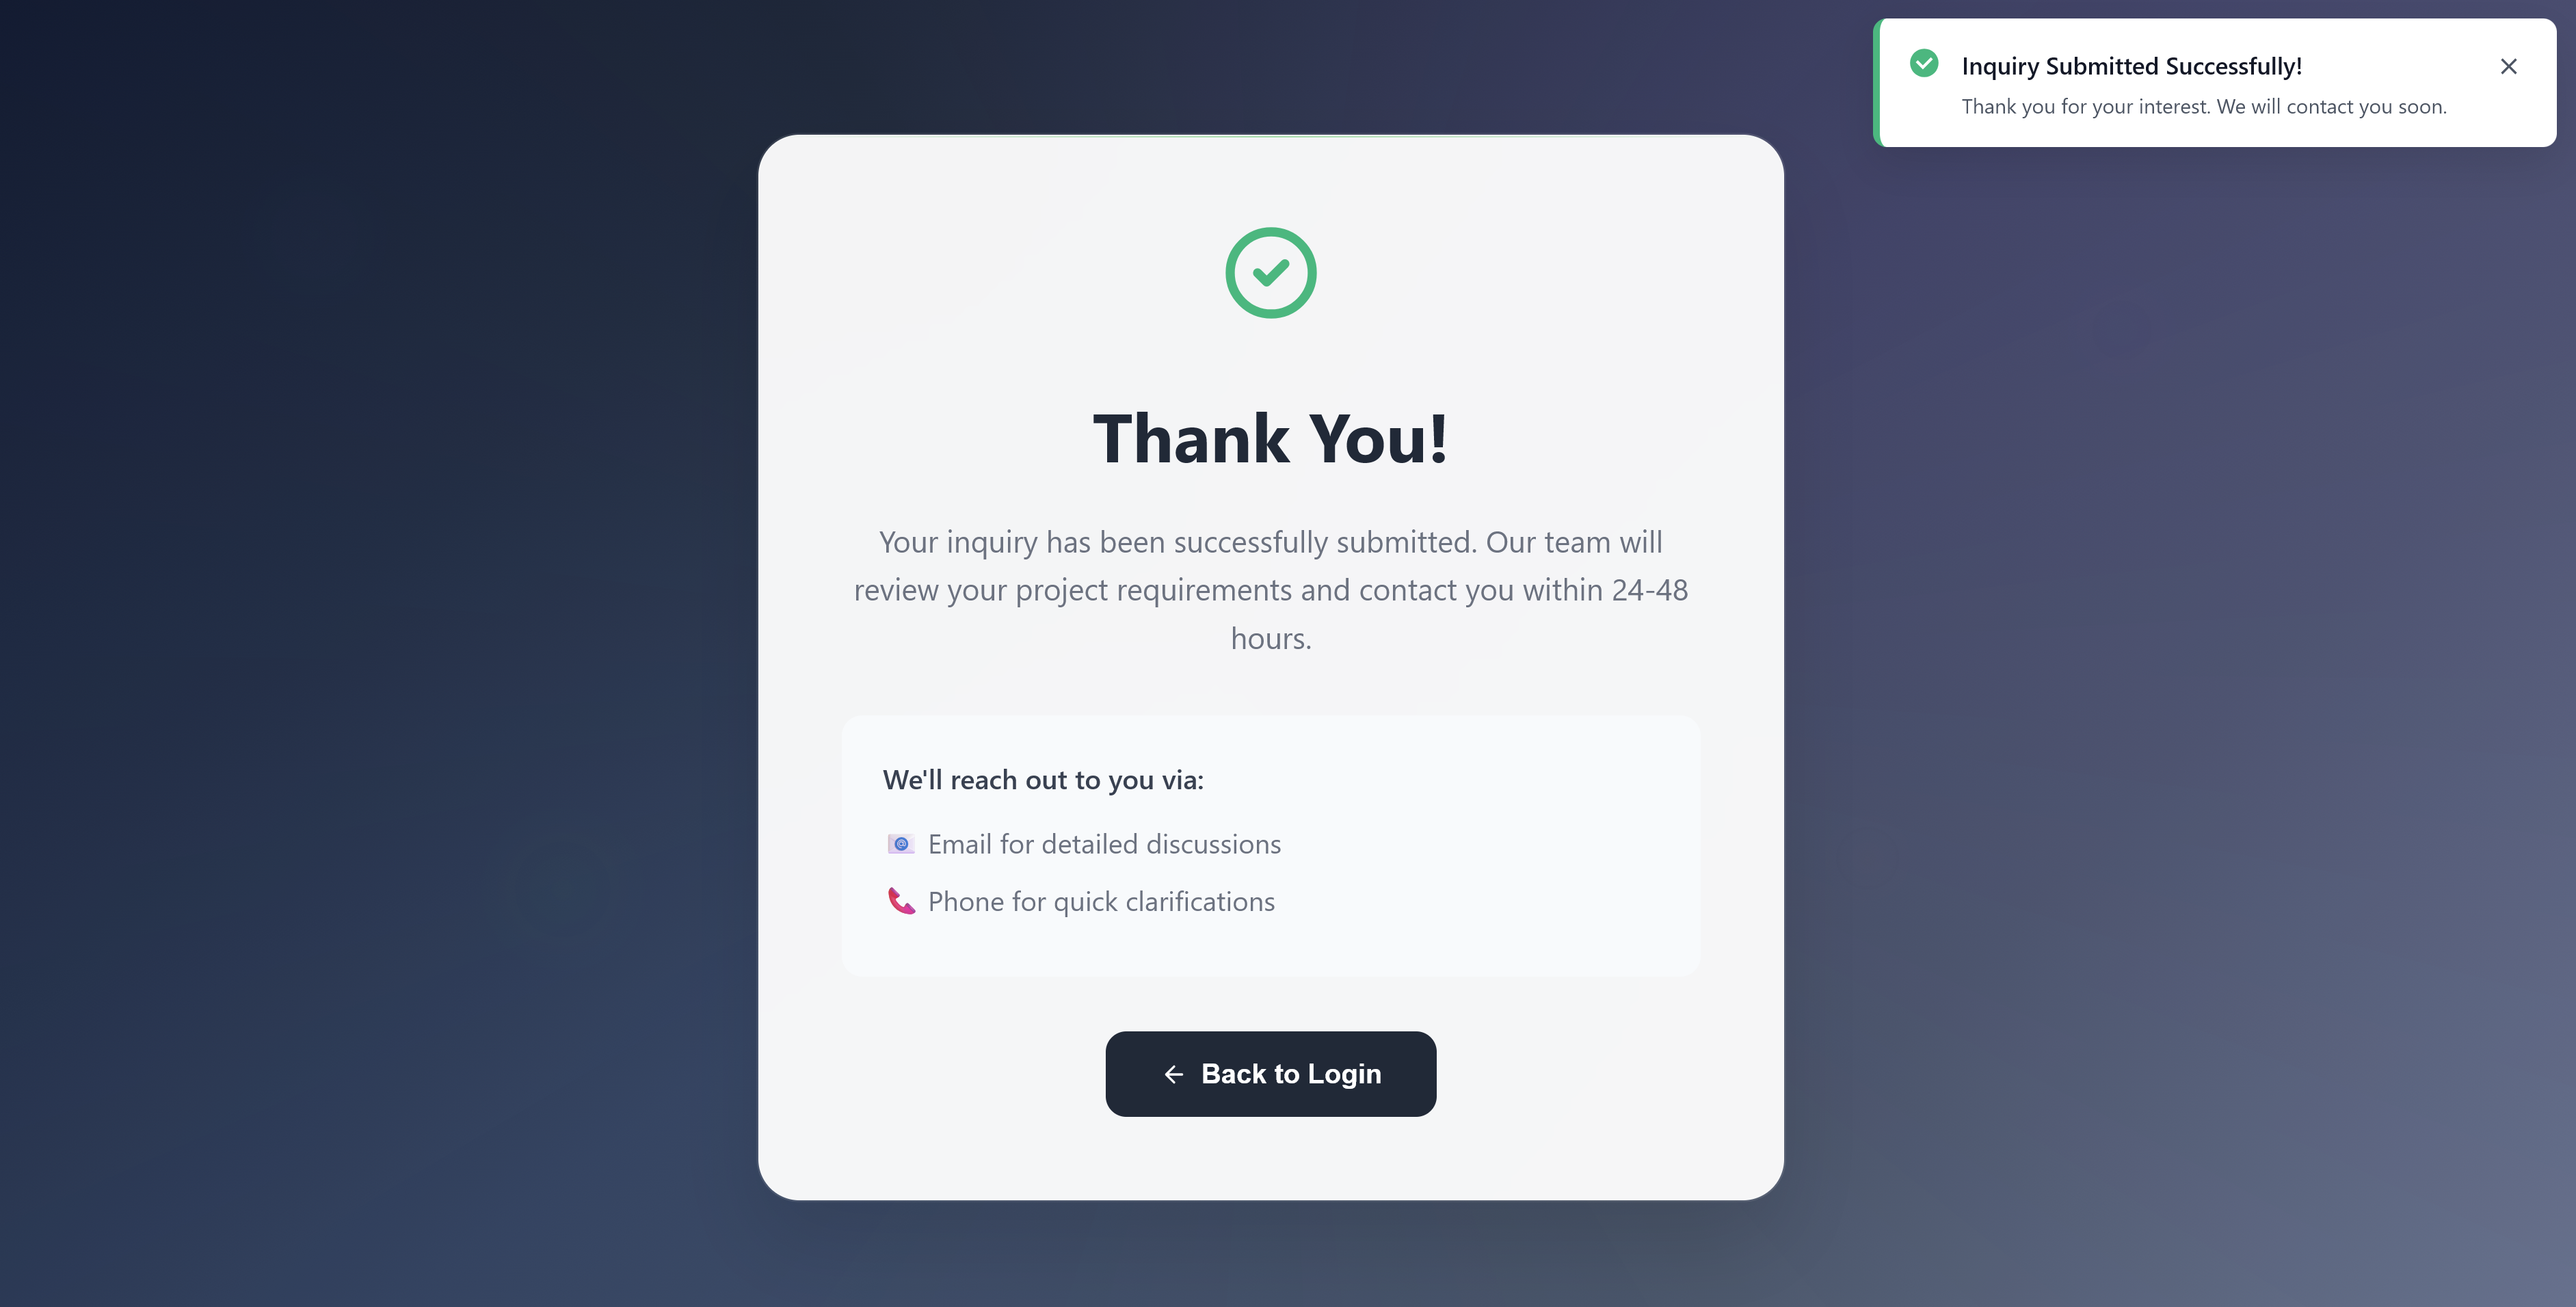
\includegraphics[width=\textwidth]{Figures/pm screenshots/client (not a real user btw)/Confirmation.png}
    \caption{Page de confirmation de soumission de demande}
    \label{fig:client-confirmation}
\end{figure}

Cette interface de confirmation assure le client que sa demande a été transmise avec succès. Elle présente un message de remerciement, confirme que l'équipe examinera les exigences du projet, et indique un délai de réponse de 24-48 heures. L'interface inclut également des informations sur les moyens de contact (email et téléphone) et une notification de succès.

\subsection{Vue Direction}

% --- Interface Client Inquiries Management ---
\begin{figure}[H]
    \centering
    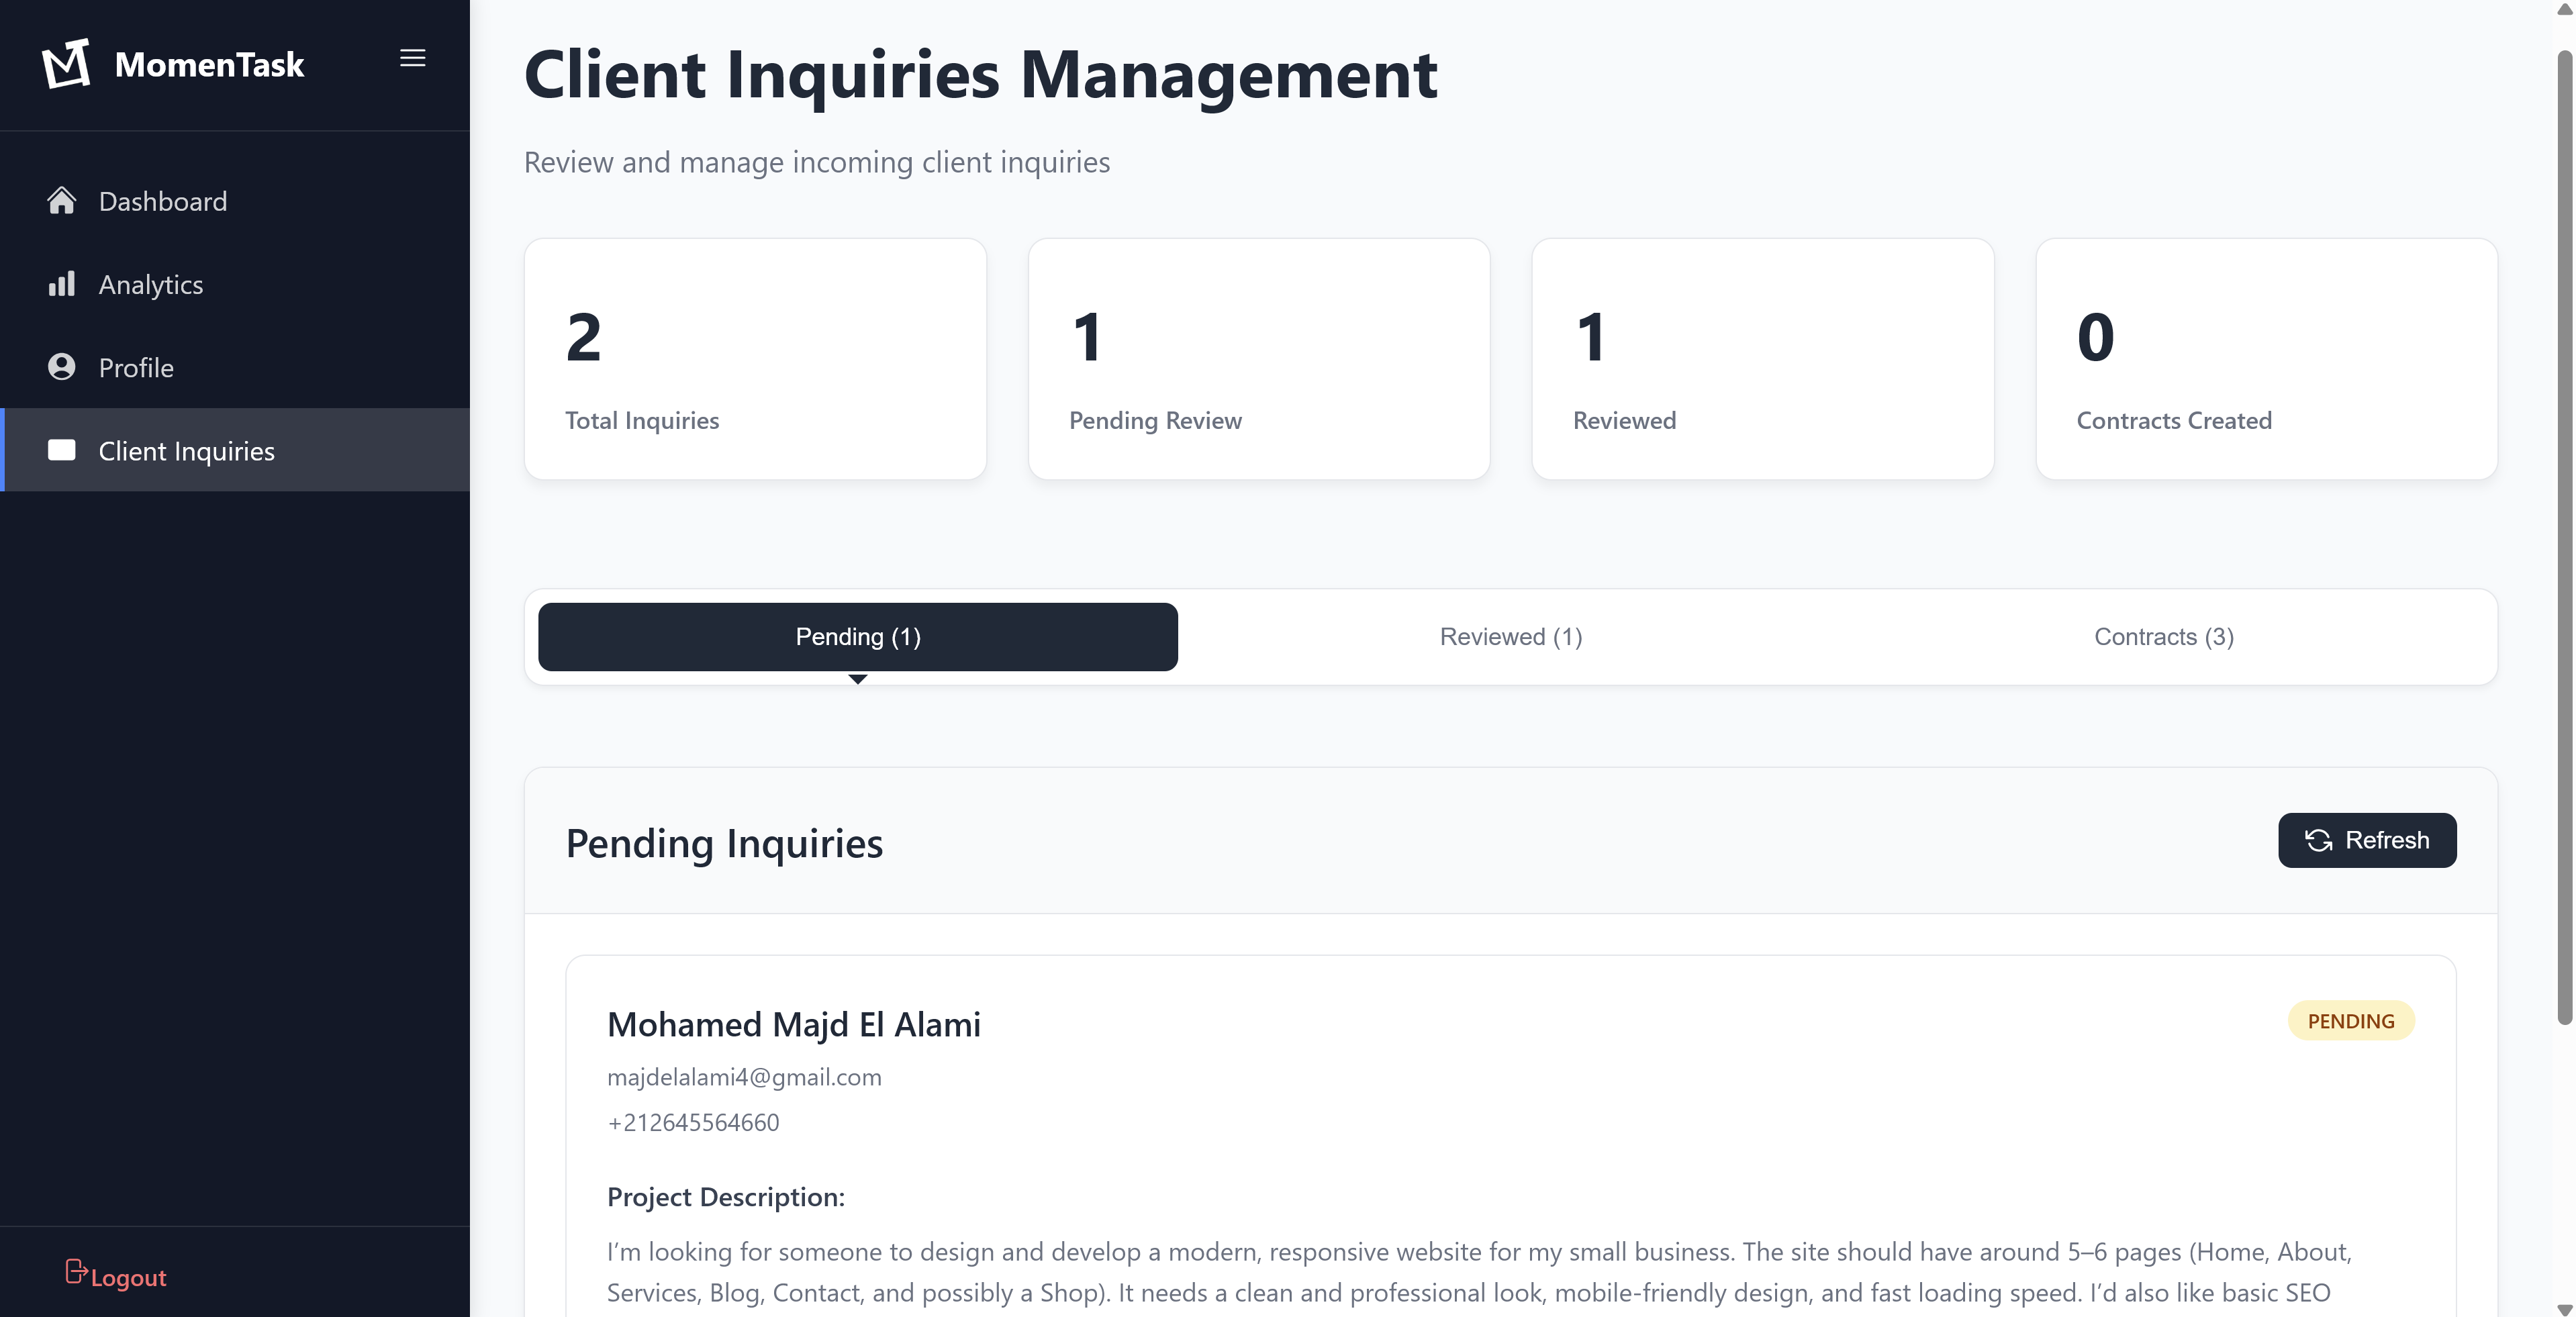
\includegraphics[width=\textwidth]{Figures/pm screenshots/direction/client inquiries management.png}
    \caption{Tableau de bord de gestion des demandes clients}
    \label{fig:direction-inquiries}
\end{figure}

Cette interface permet à la direction de gérer et suivre toutes les demandes clients entrantes. Elle présente des métriques clés (total des demandes, en attente, examinées, contrats créés) et organise les demandes par statut. L'interface affiche les détails complets de chaque demande, incluant les informations de contact et la description du projet, facilitant ainsi le processus de revue et de prise de décision.

% --- Interface Contrat ---
\begin{figure}[H]
    \centering
    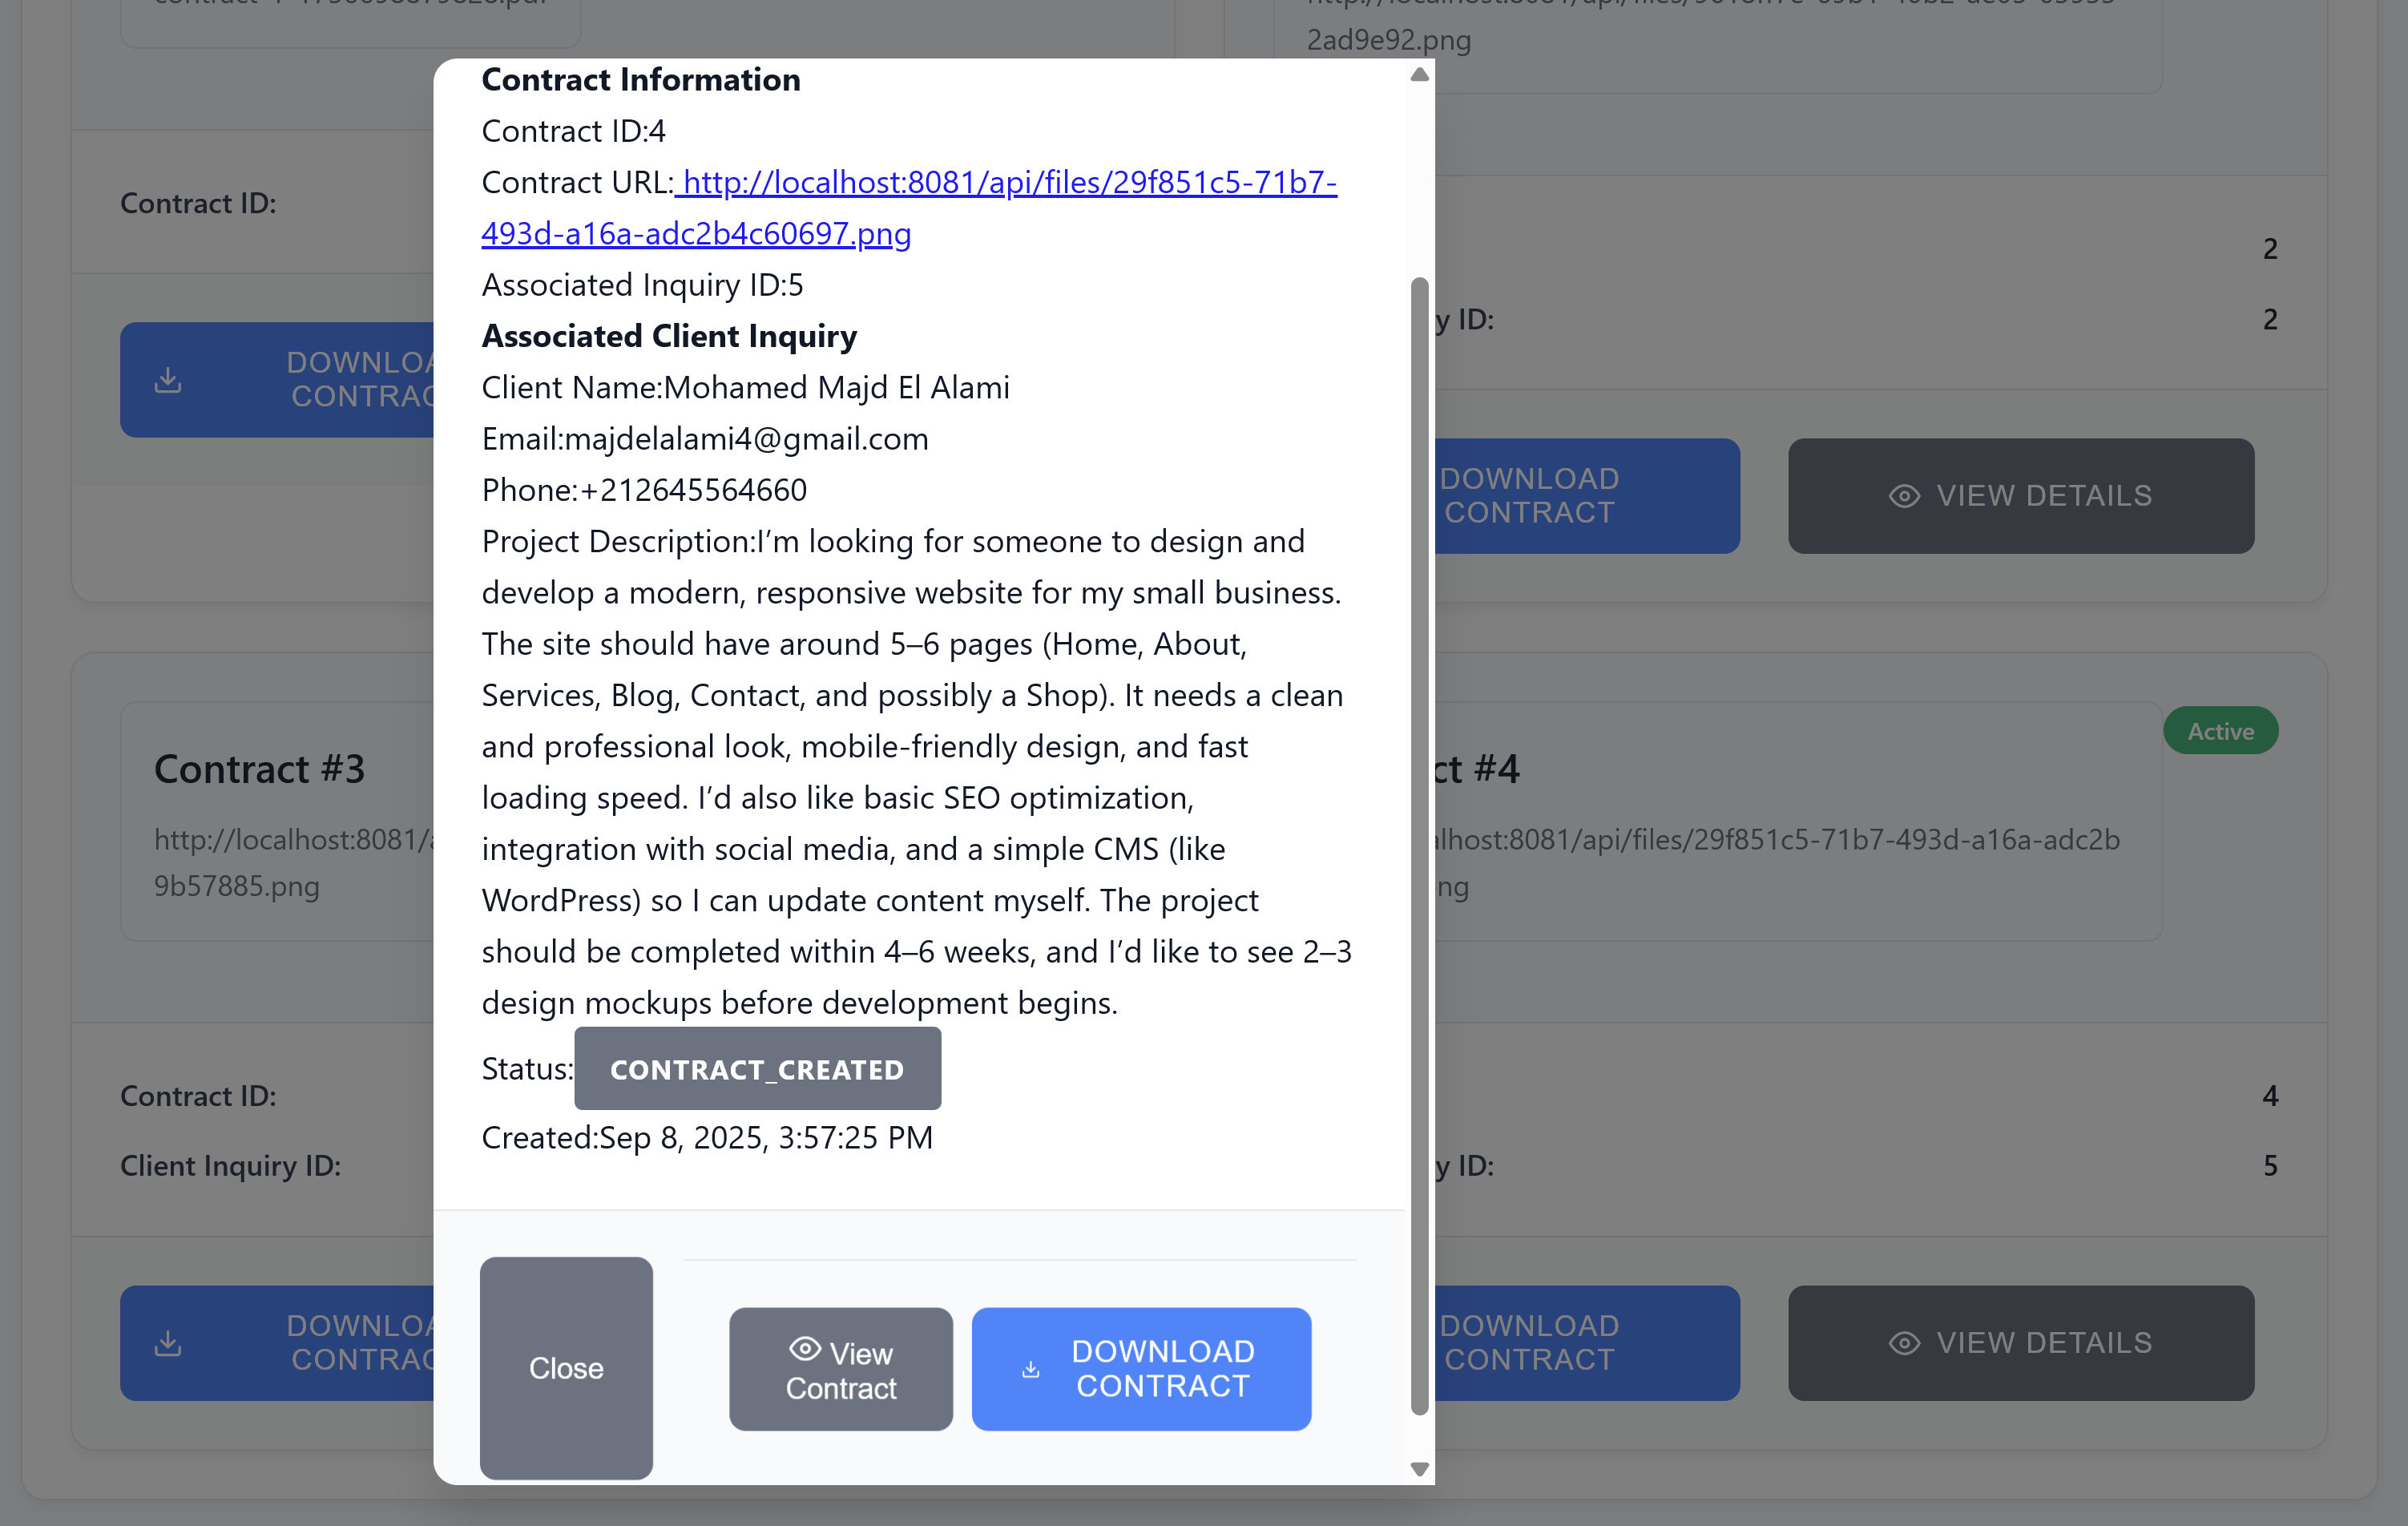
\includegraphics[width=\textwidth]{Figures/pm screenshots/direction/contrat.png}
    \caption{Interface de gestion des contrats et modal de détails}
    \label{fig:direction-contrat}
\end{figure}

Cette interface de gestion des contrats permet à la direction de visualiser et gérer tous les contrats créés. Elle affiche une liste de contrats avec leurs identifiants, URLs, et statuts. Le modal de détails montre les informations complètes du contrat, incluant les détails de la demande client associée, le statut de création, et les options de téléchargement et de visualisation.

% --- Interface Statistiques ---
\begin{figure}[H]
    \centering
    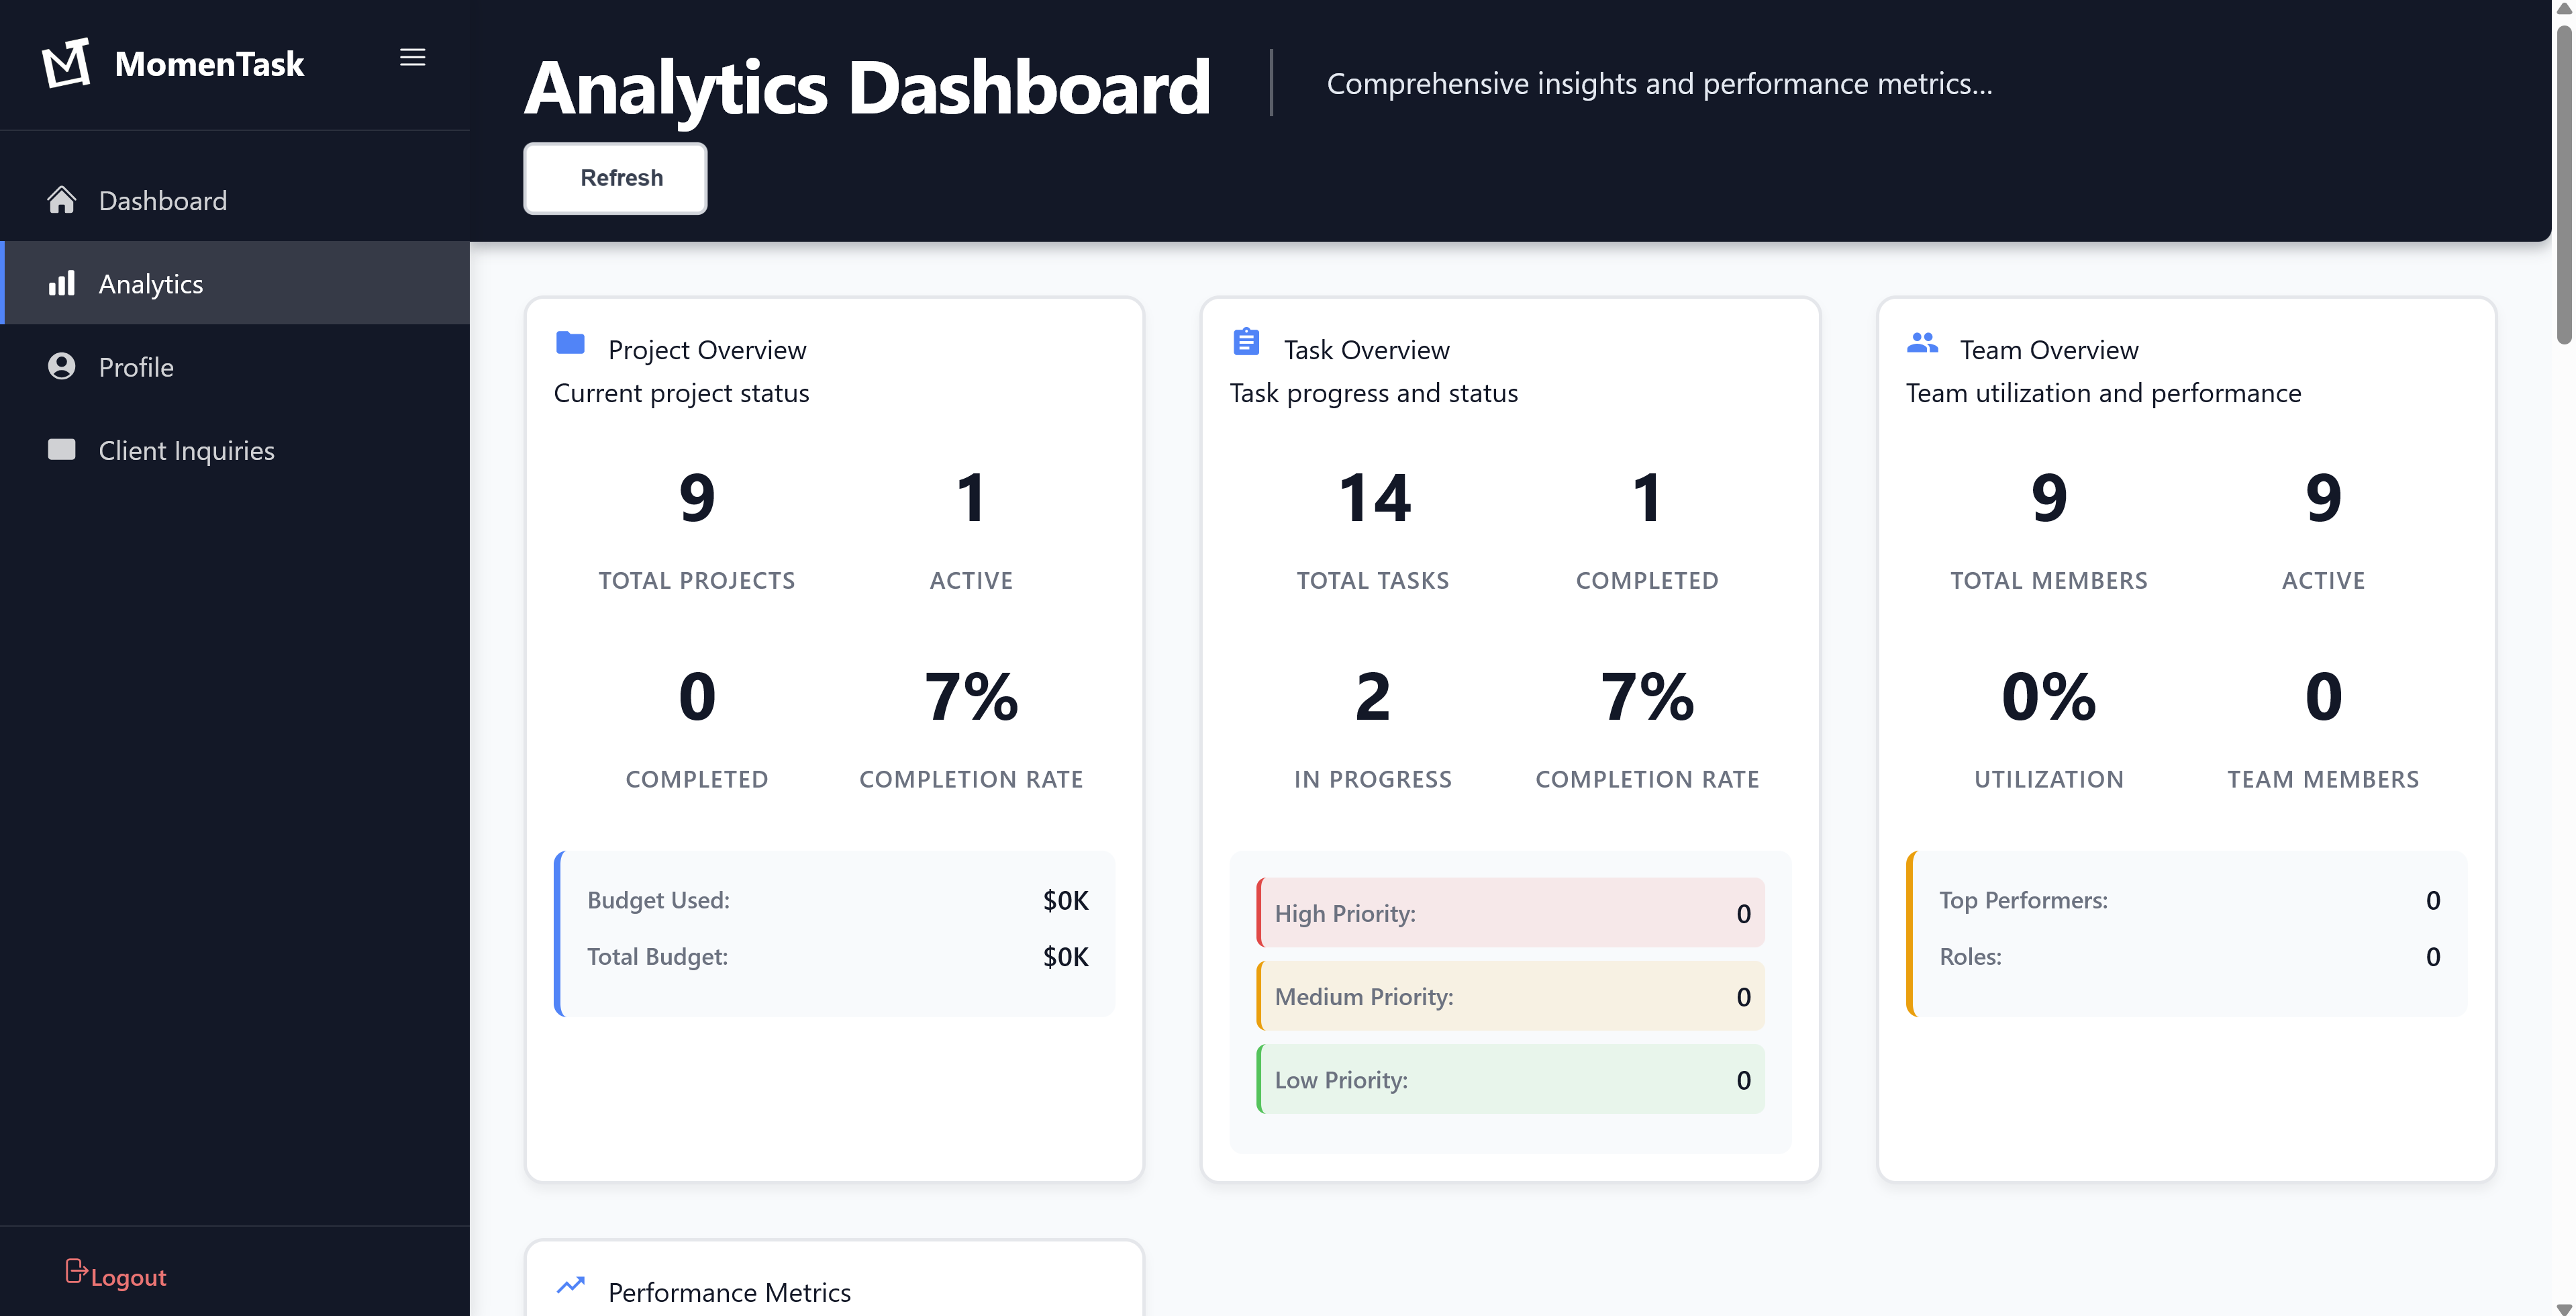
\includegraphics[width=\textwidth]{Figures/pm screenshots/direction/statistiques.png}
    \caption{Tableau de bord analytique avec métriques de performance}
    \label{fig:direction-statistiques}
\end{figure}

Cette interface analytique fournit à la direction une vue d'ensemble des performances du portefeuille de projets. Elle présente des métriques clés : aperçu des projets (total, actifs, complétés, taux de completion), aperçu des tâches (total, complétées, en cours), et aperçu de l'équipe (membres totaux, actifs, taux d'utilisation). Ces données permettent un suivi décisionnel efficace.

\subsection{Vue IT ADMIN}

% --- Interface User Management ---
\begin{figure}[H]
    \centering
    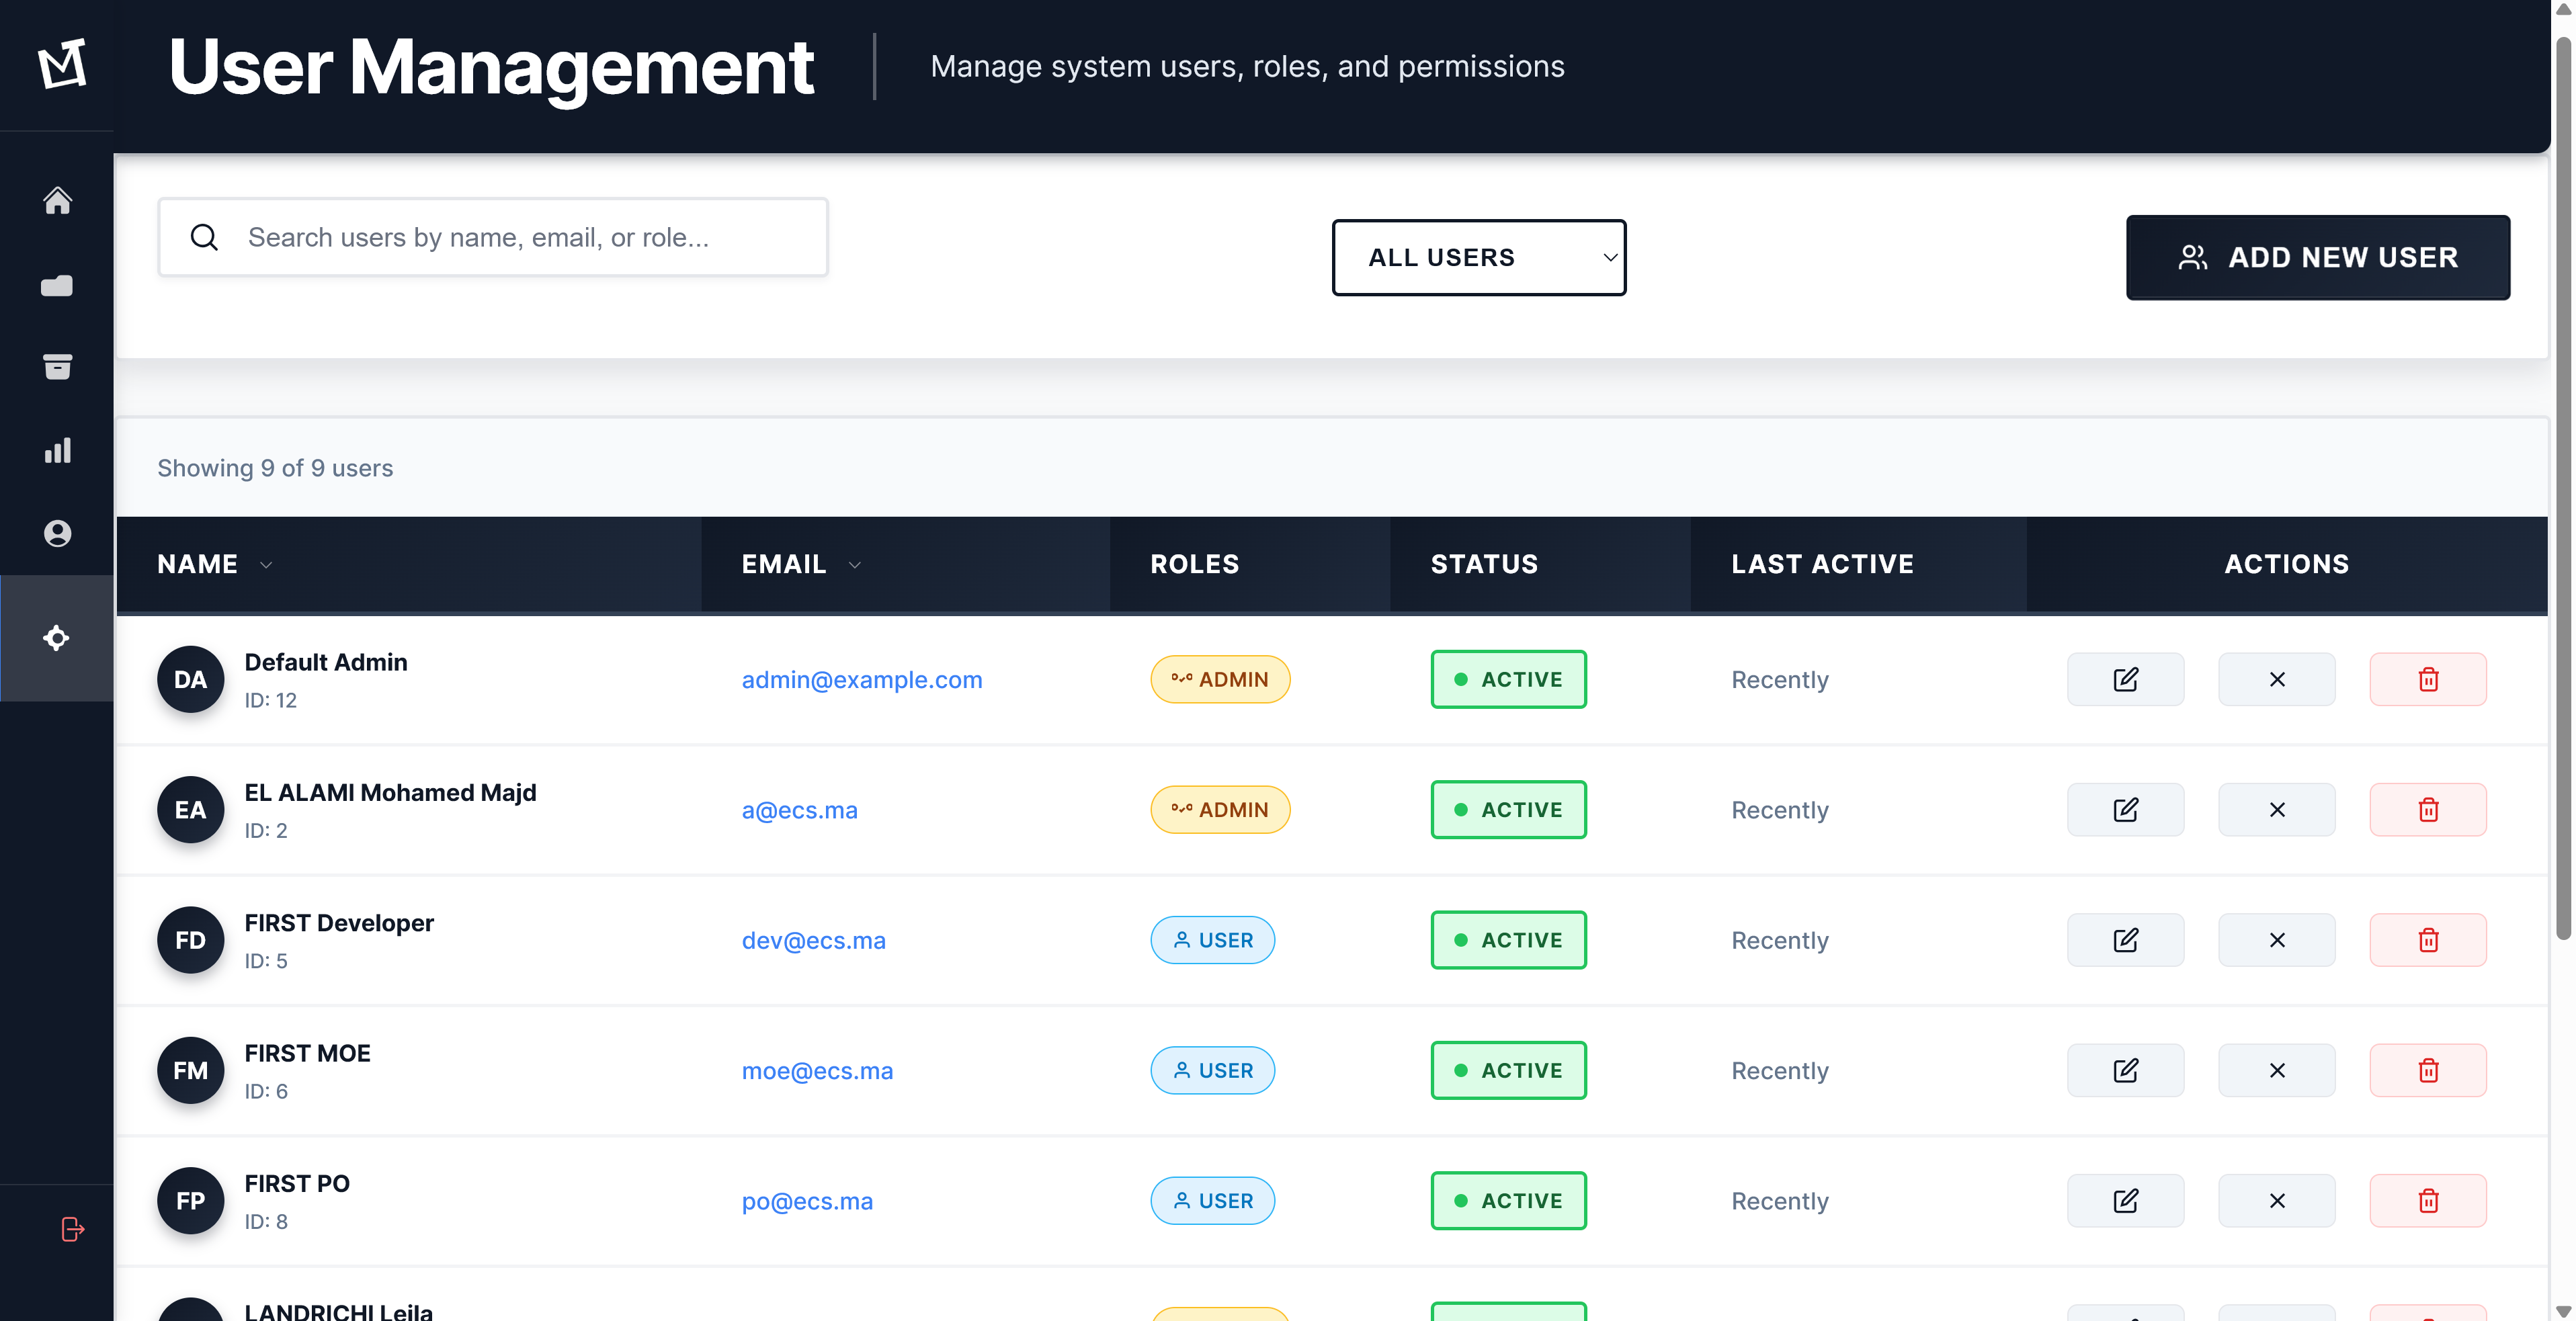
\includegraphics[width=\textwidth]{Figures/pm screenshots/admin/user management.png}
    \caption{Interface de gestion des utilisateurs et des rôles système}
    \label{fig:admin-users}
\end{figure}

Cette interface permet à l'administrateur IT de gérer tous les utilisateurs du système. Elle affiche une liste complète des utilisateurs avec leurs informations (nom, email, rôles, statut, dernière activité) et propose des actions de gestion (édition, suppression). La barre de recherche et les filtres facilitent la navigation dans une base d'utilisateurs importante.

% --- Interface Edit User ---
\begin{figure}[H]
    \centering
    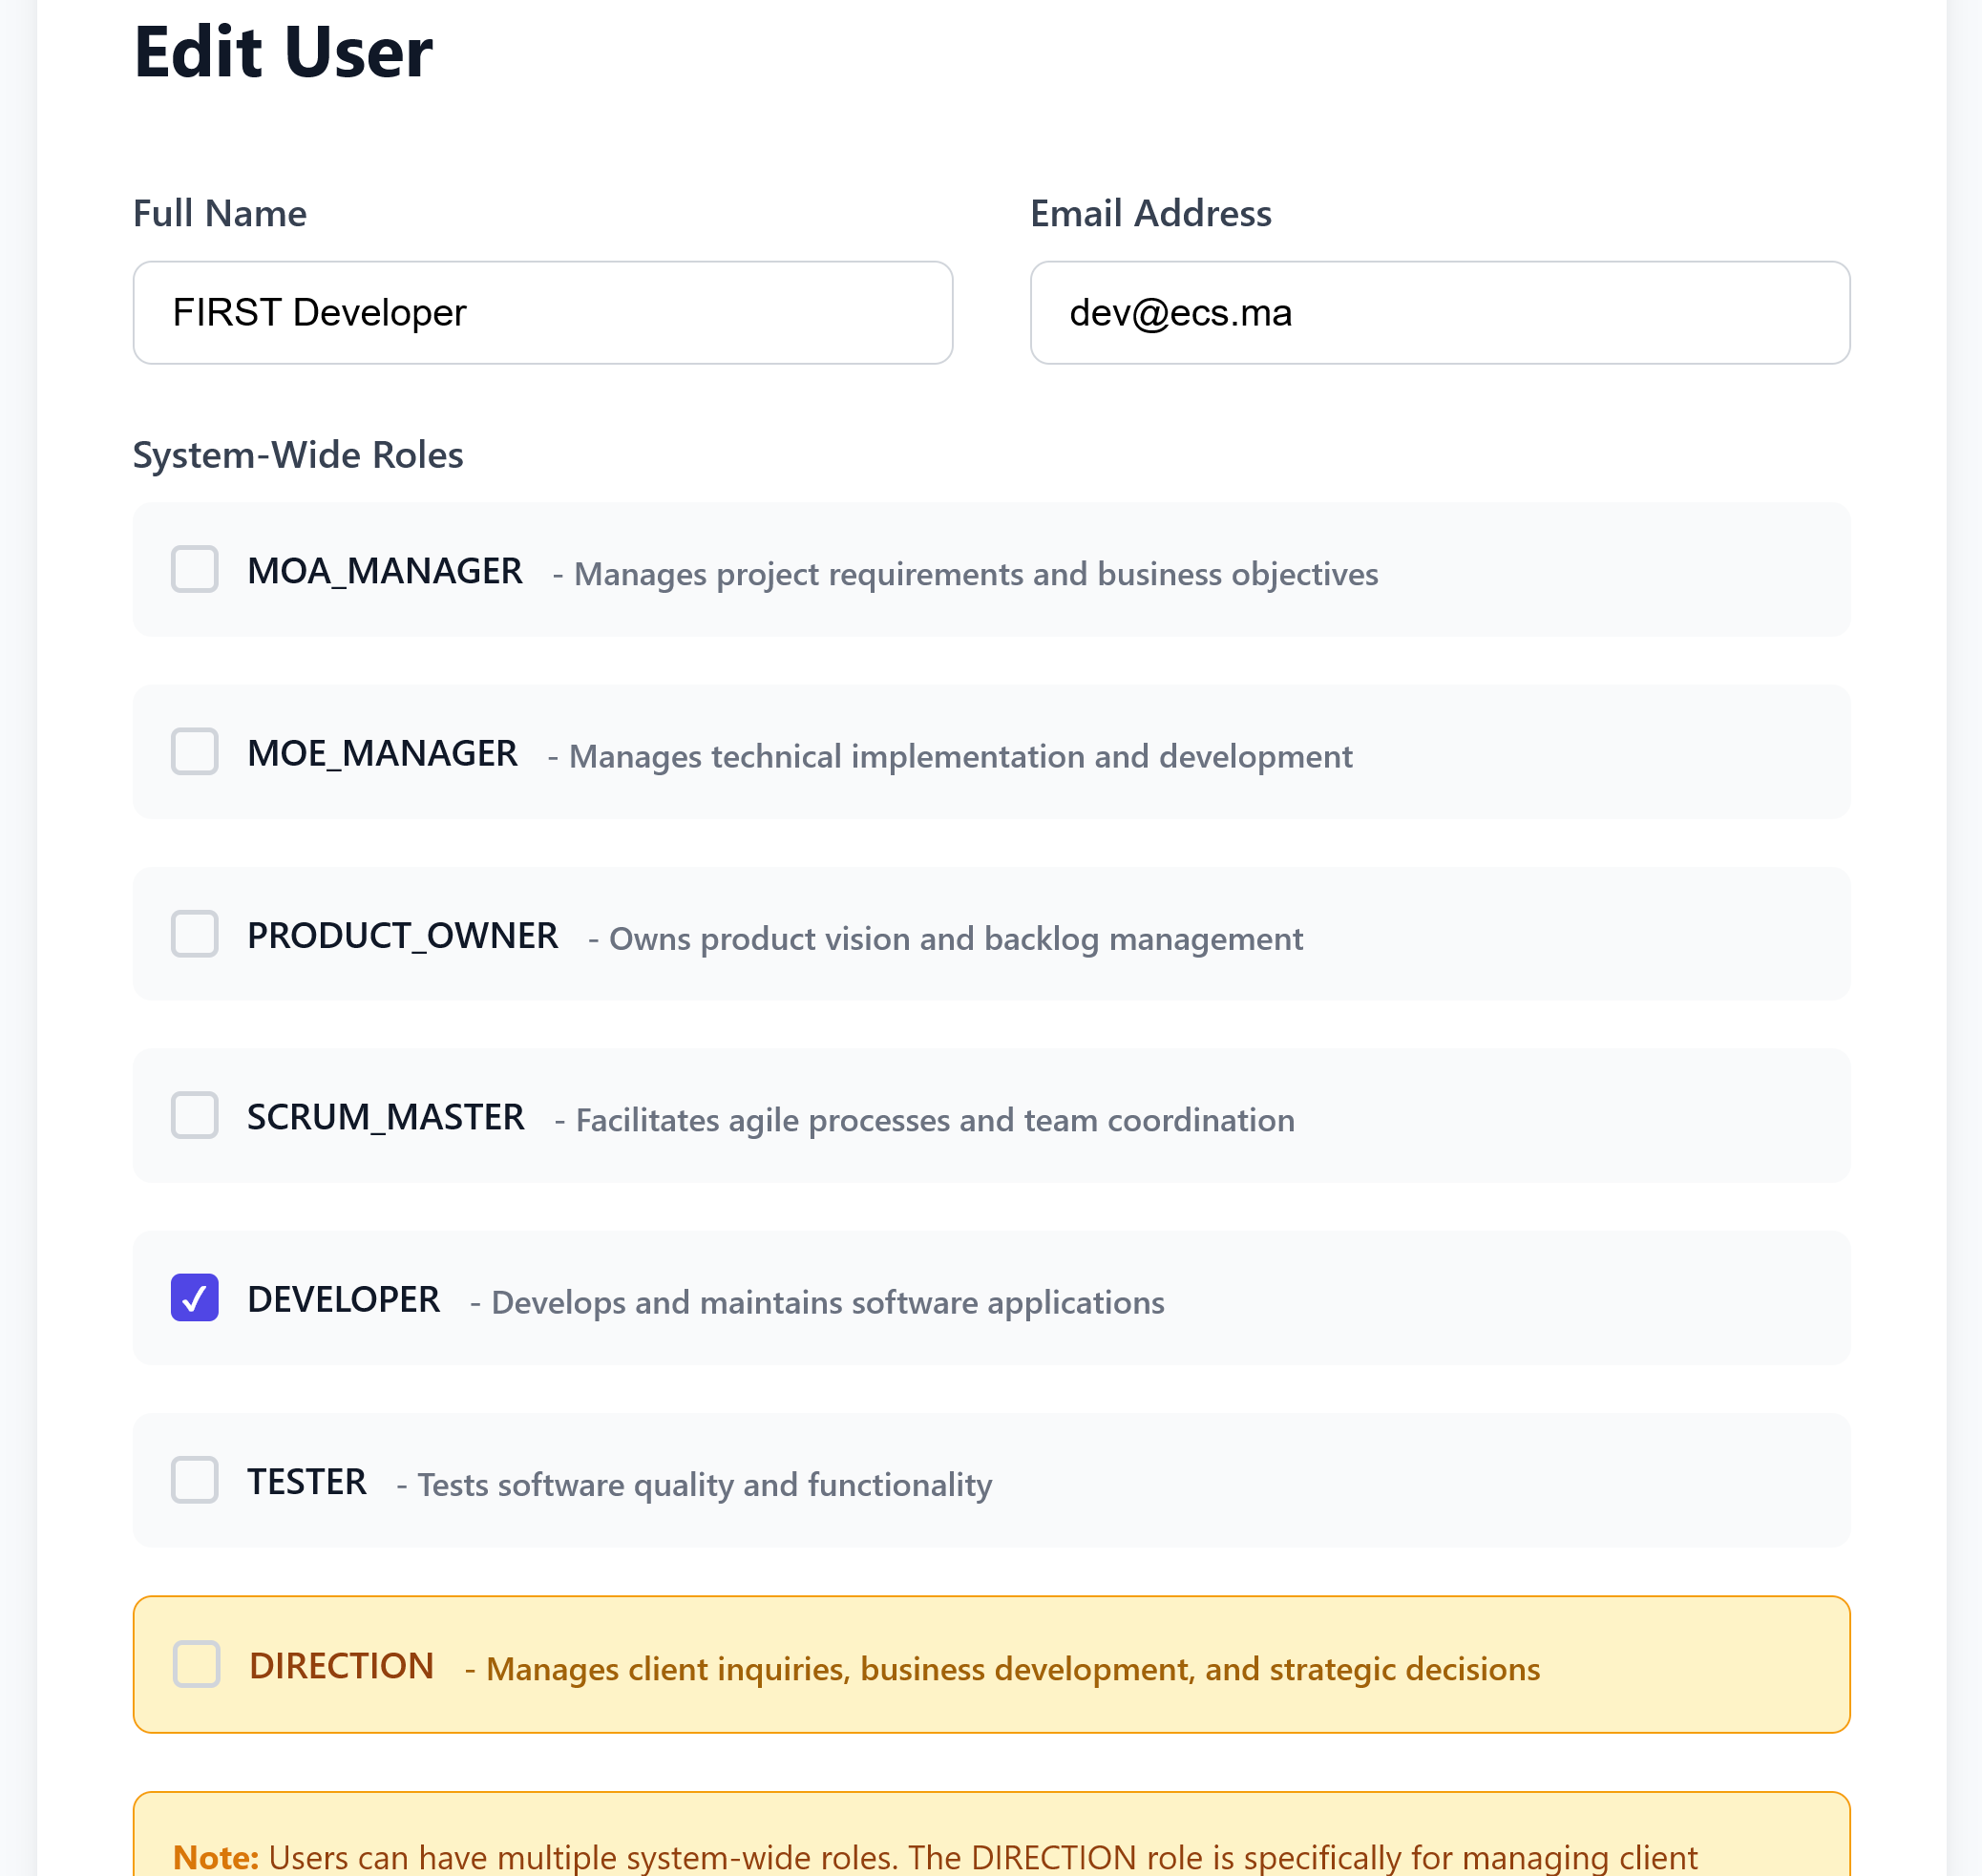
\includegraphics[width=\textwidth]{Figures/pm screenshots/admin/edit user (roles..).png}
    \caption{Formulaire d'édition des utilisateurs et attribution des rôles}
    \label{fig:admin-edit-user}
\end{figure}

Cette interface permet de modifier les informations d'un utilisateur et de gérer ses rôles système. Elle présente les rôles disponibles (MOA\_MANAGER, MOE\_MANAGER, PRODUCT\_OWNER, SCRUM\_MASTER, DEVELOPER, TESTER, DIRECTION) avec leurs descriptions, permettant une attribution précise des permissions selon les responsabilités de chaque utilisateur.

% --- Interface Resource Management ---
\begin{figure}[H]
    \centering
    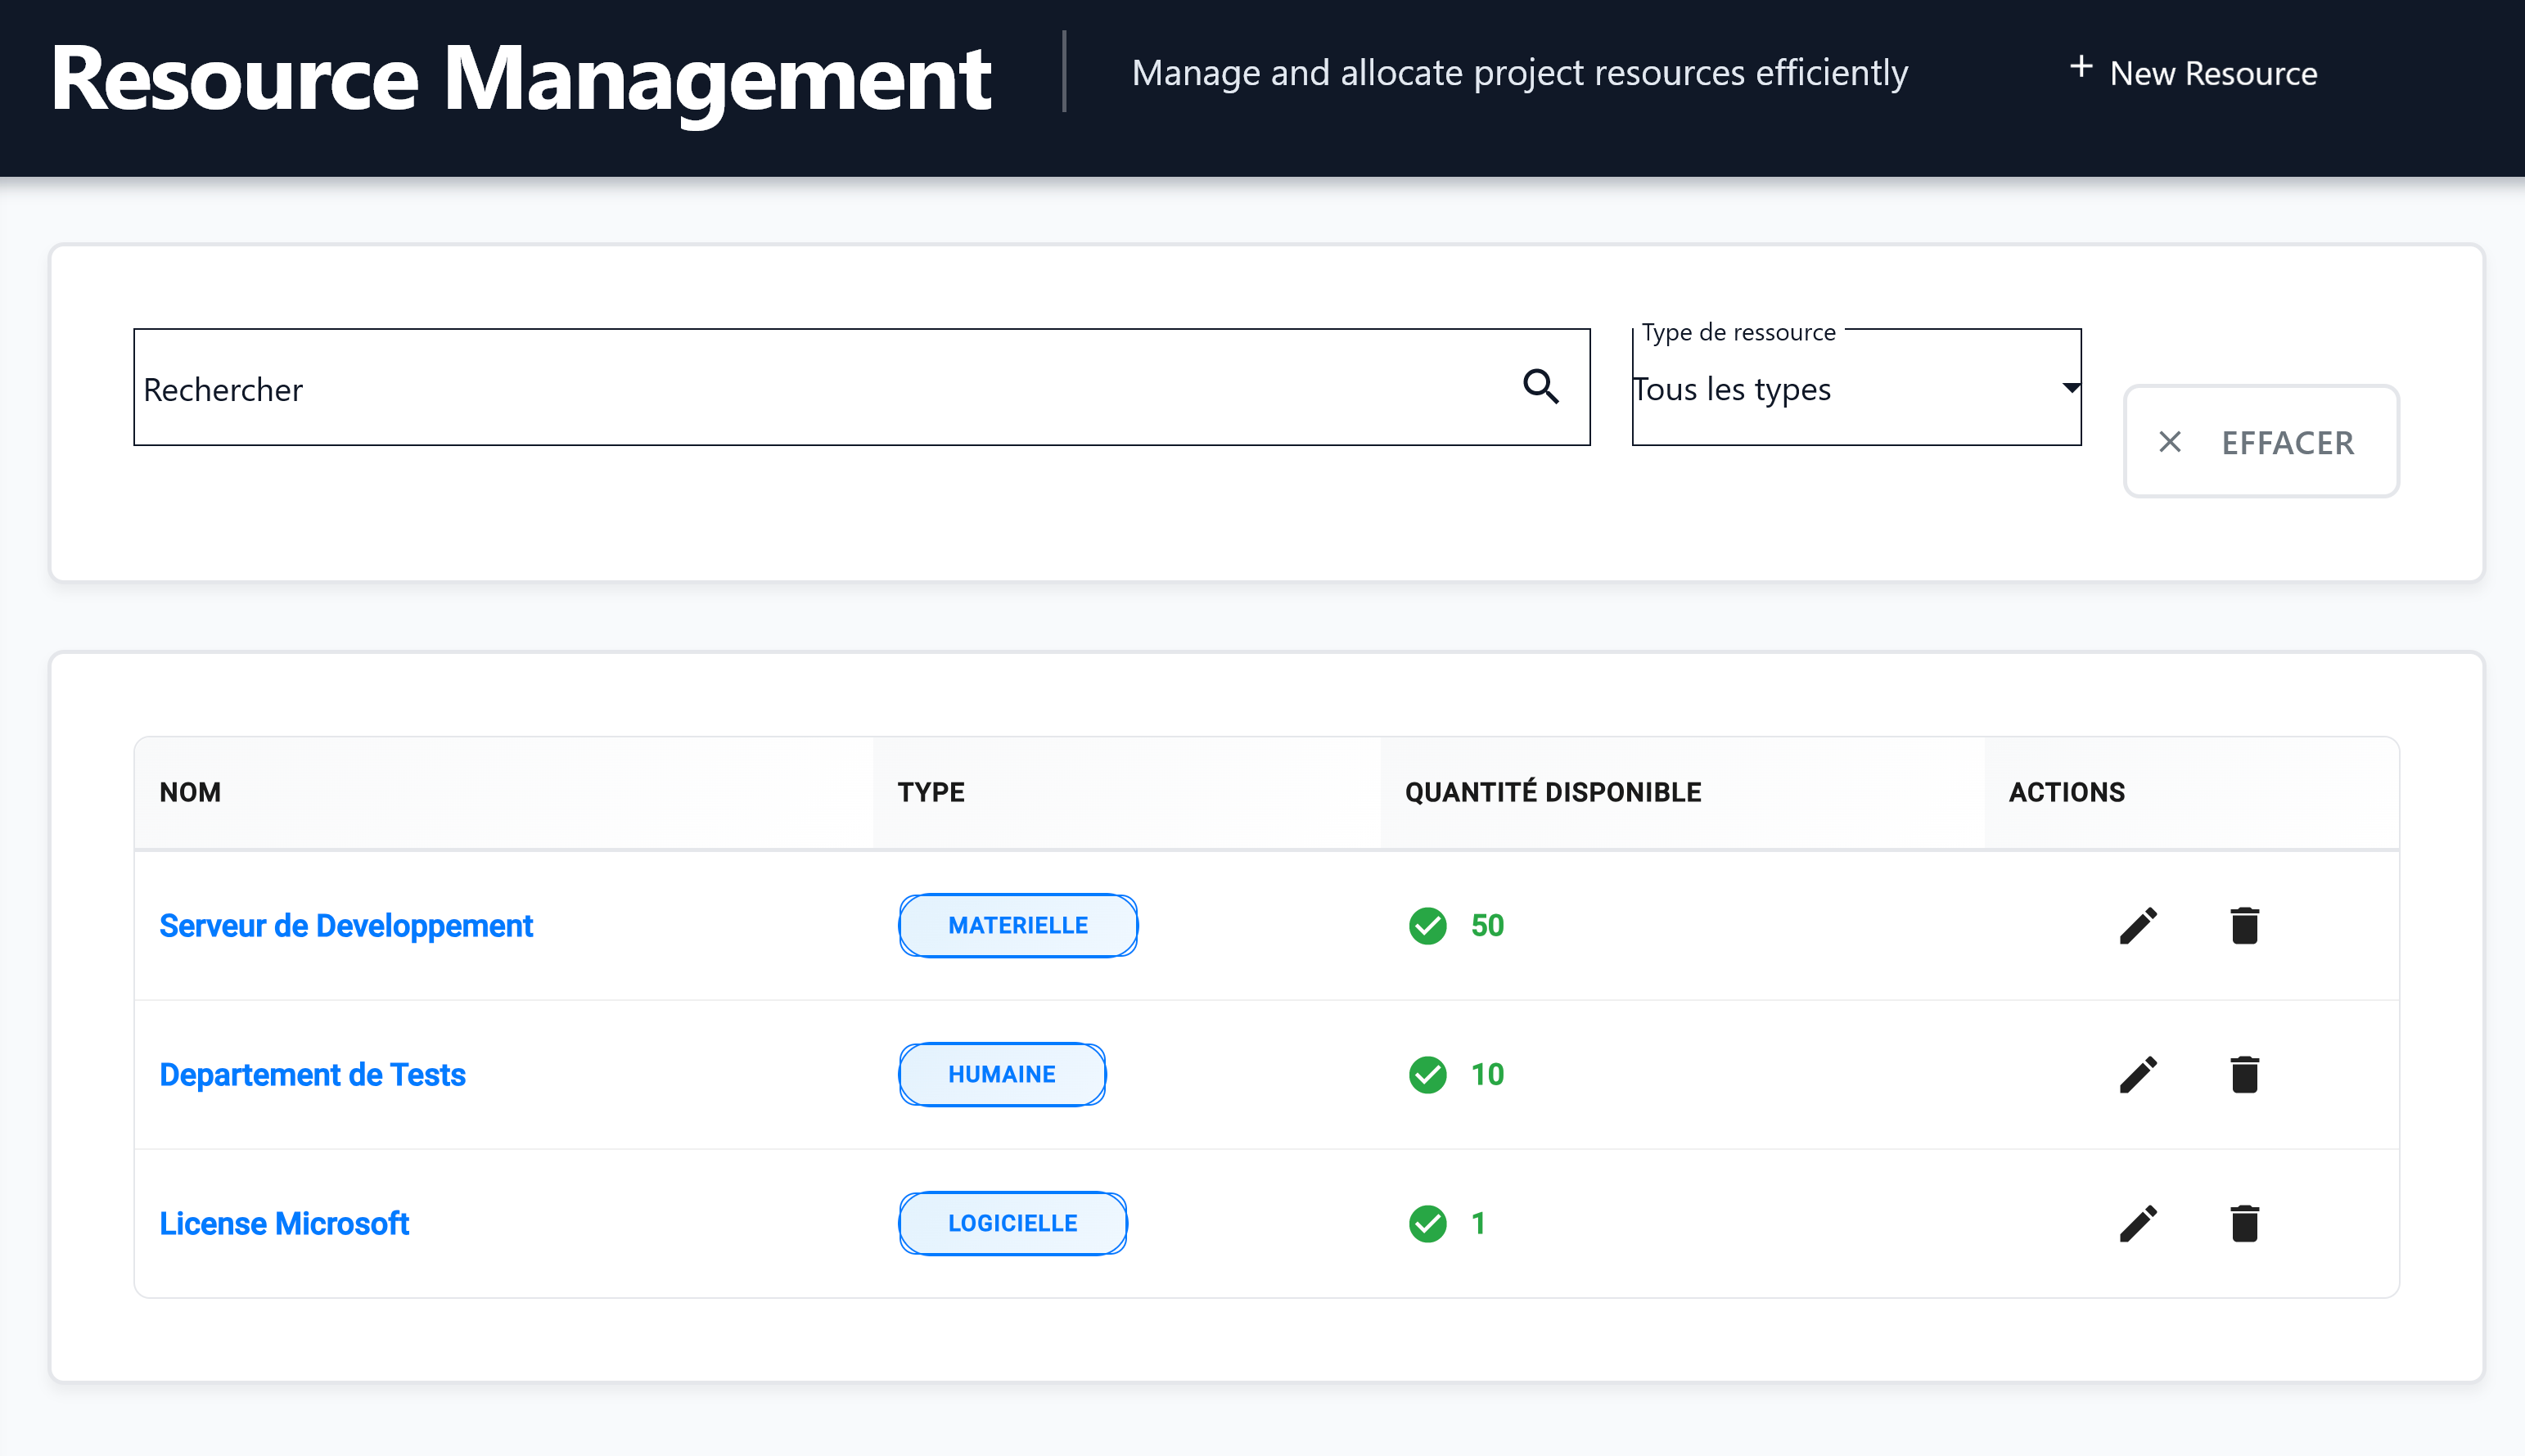
\includegraphics[width=\textwidth]{Figures/pm screenshots/admin/ressource management.png}
    \caption{Interface de gestion des ressources projet}
    \label{fig:admin-resources}
\end{figure}

Cette interface permet de gérer les ressources allouées aux projets, qu'elles soient matérielles, humaines ou logicielles. Elle affiche la liste des ressources avec leur type, quantité disponible, et propose des actions de gestion. Les ressources incluent des serveurs de développement, des départements de tests, et des licences logicielles, facilitant ainsi la planification et l'allocation des moyens.

\subsection{Vue Product Owner (SCRUM)}

% --- Interface Backlog ---
\begin{figure}[H]
    \centering
    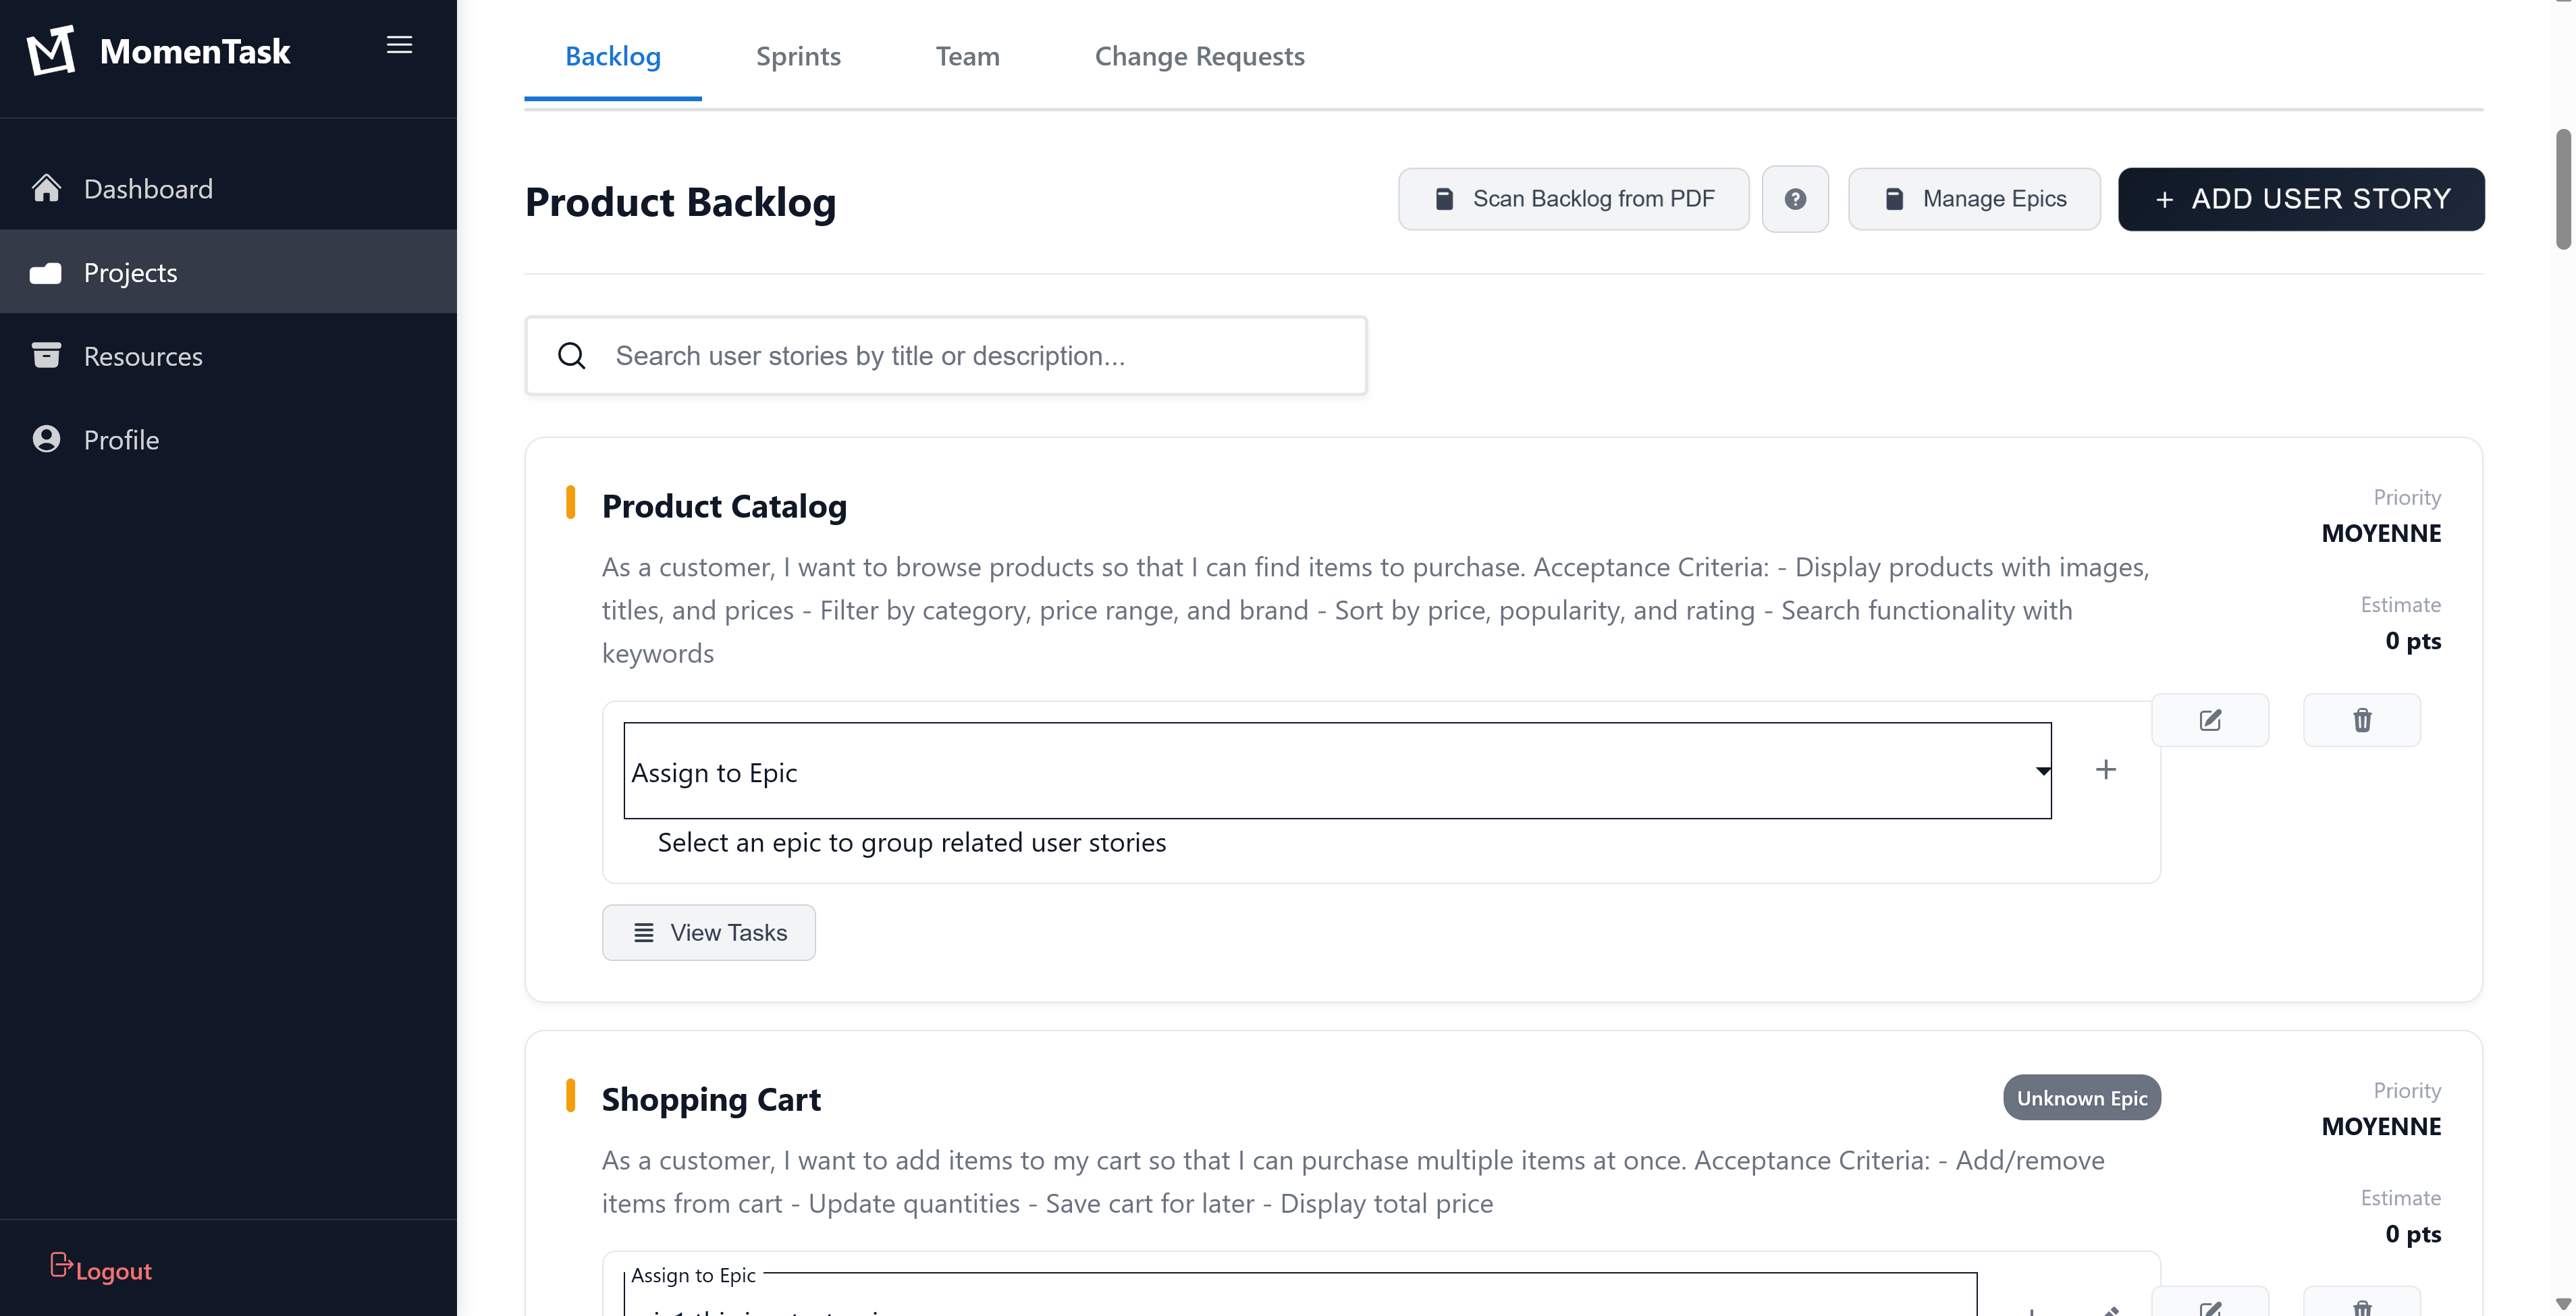
\includegraphics[width=\textwidth]{Figures/pm screenshots/po/backlog.png}
    \caption{Interface de gestion du backlog produit}
    \label{fig:po-backlog}
\end{figure}

Cette interface permet au Product Owner de gérer le backlog produit. Elle présente les user stories avec leurs descriptions détaillées, critères d'acceptation, priorités et estimations. L'interface propose des fonctionnalités de recherche, d'assignation aux epics, et de visualisation des tâches associées, facilitant ainsi la planification et la priorisation des fonctionnalités.

\subsection{Vue Scrum Master}

% --- Interface Team Management ---
\begin{figure}[H]
    \centering
    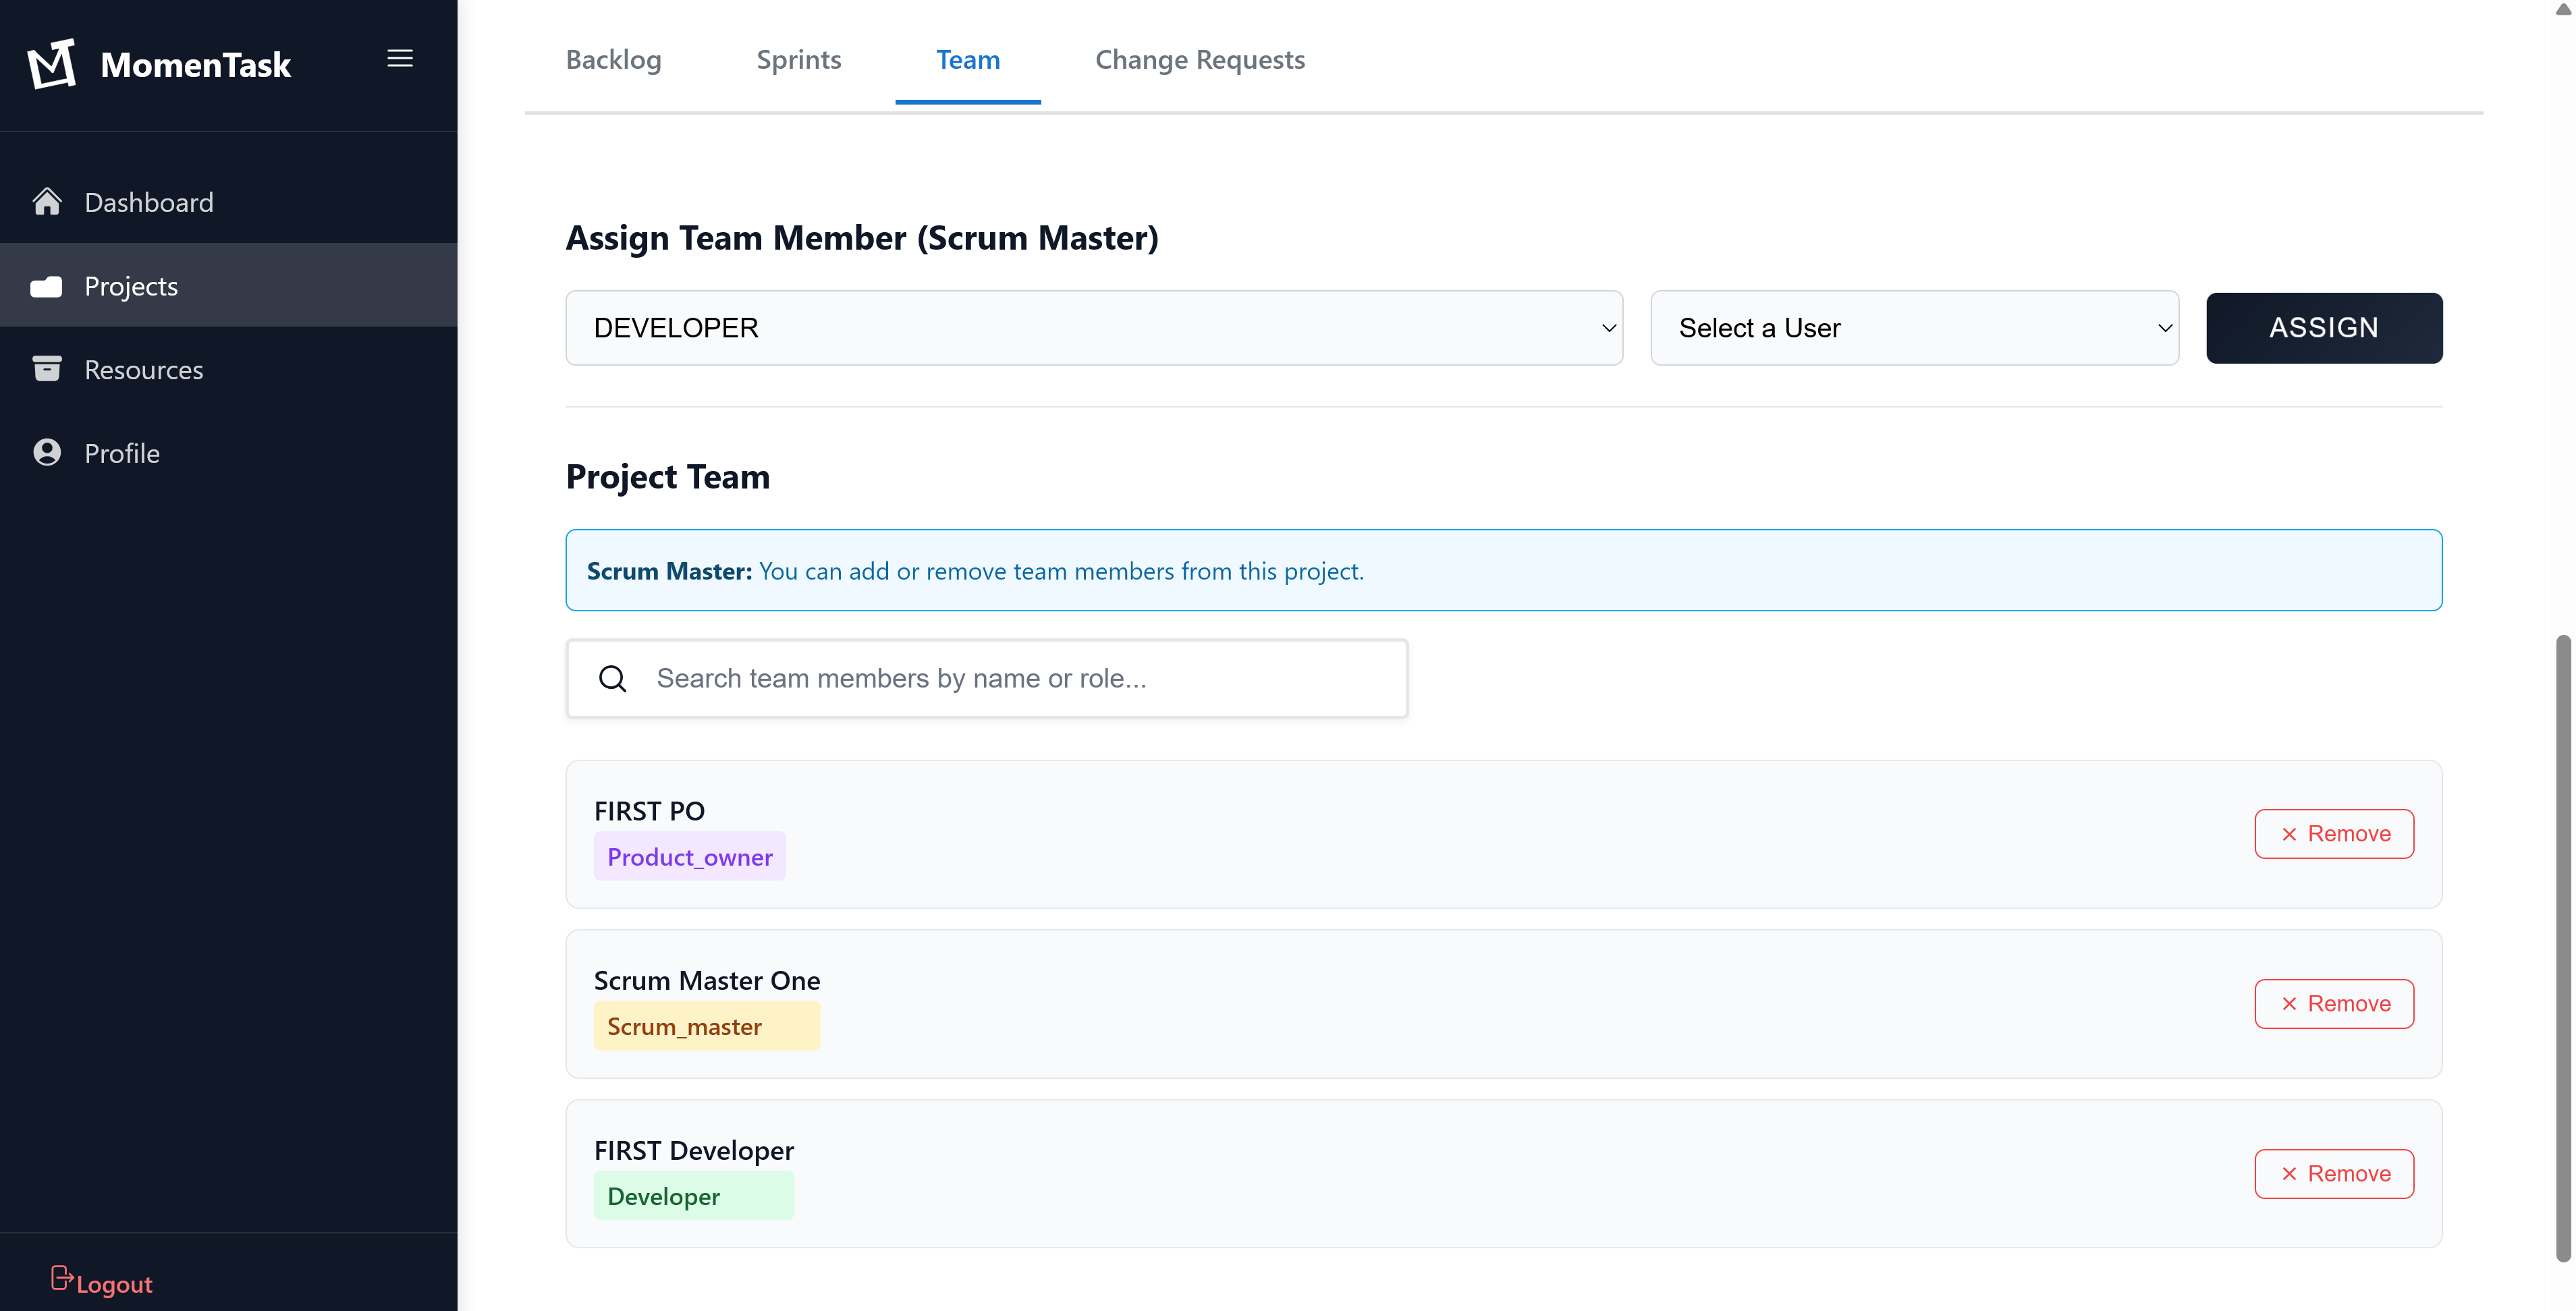
\includegraphics[width=\textwidth]{Figures/pm screenshots/scrummaster/team.png}
    \caption{Interface de gestion de l'équipe projet}
    \label{fig:scrummaster-team}
\end{figure}

Cette interface permet au Scrum Master de gérer l'équipe du projet. Elle propose des fonctionnalités d'assignation de membres d'équipe avec attribution de rôles spécifiques, de recherche dans l'équipe existante, et de visualisation des membres actuels avec leurs rôles respectifs. L'interface facilite la constitution et la gestion des équipes de développement.

\subsection{Vue Développeur}

% --- Interface Change Requests ---
\begin{figure}[H]
    \centering
    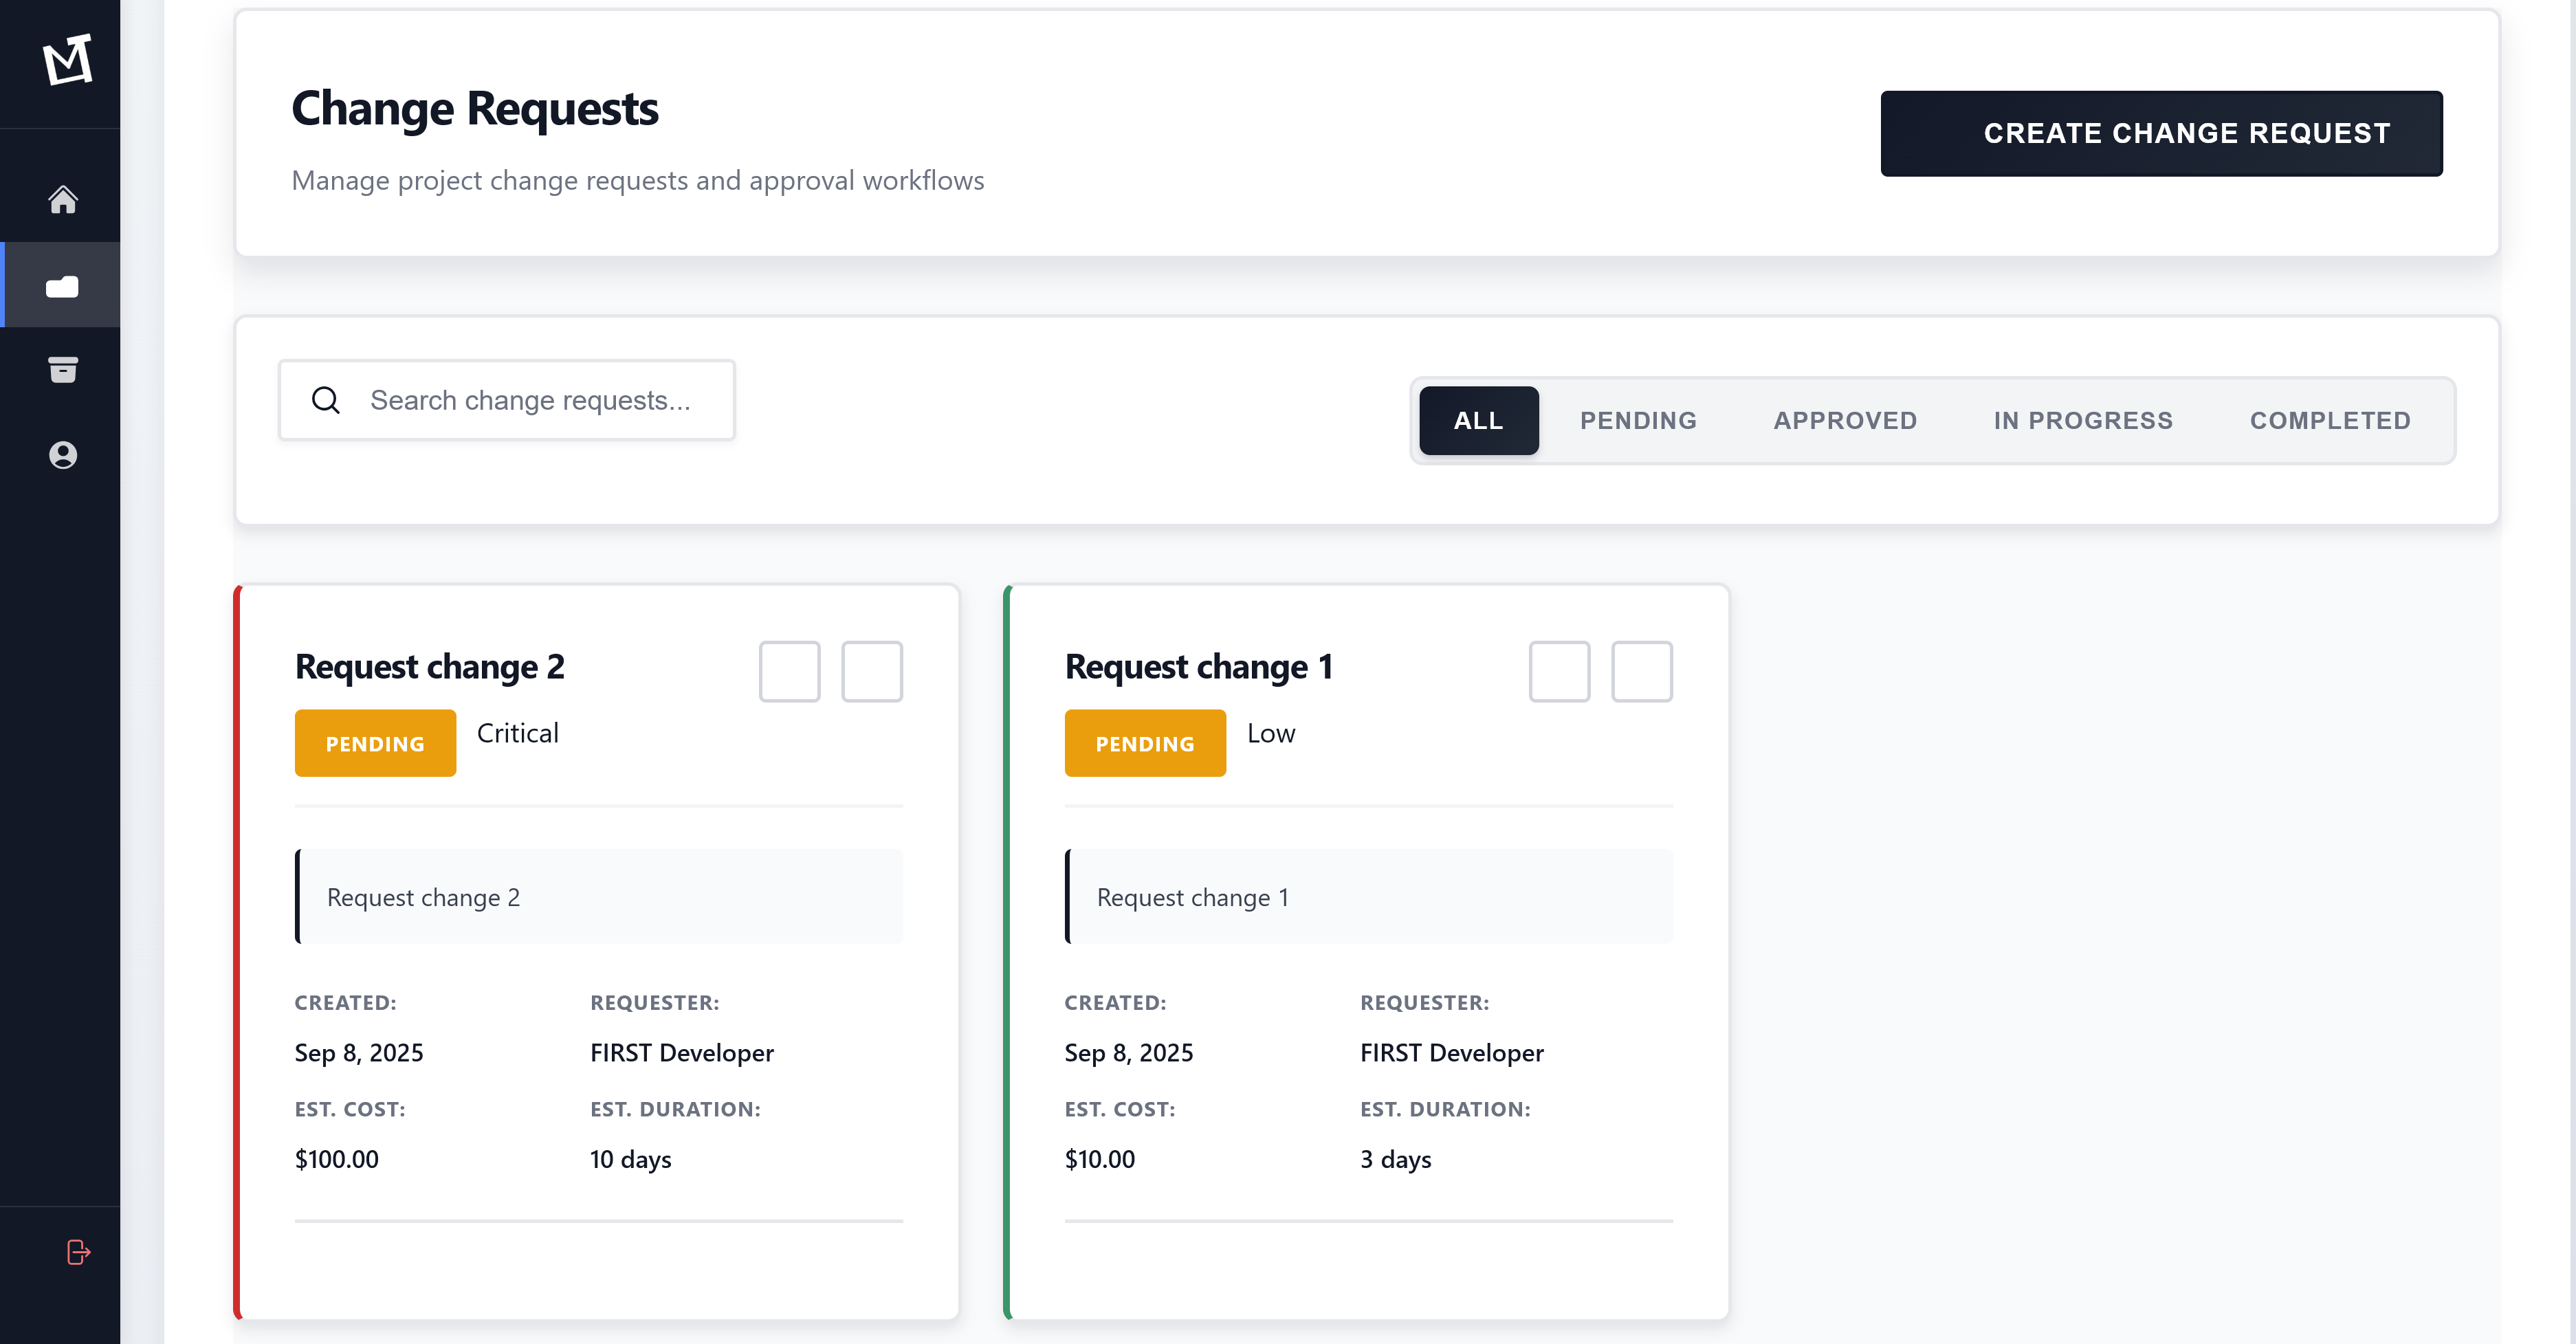
\includegraphics[width=\textwidth]{Figures/pm screenshots/dev/change requests.png}
    \caption{Interface de gestion des demandes de changement}
    \label{fig:dev-change-requests}
\end{figure}

Cette interface permet aux développeurs de gérer les demandes de changement du projet. Elle affiche les demandes avec leurs statuts (PENDING, APPROVED, IN PROGRESS, COMPLETED), priorités, et détails (coût estimé, durée, demandeur). L'interface propose des filtres par statut et des fonctionnalités de recherche pour un suivi efficace des modifications.

% --- Interface Dashboard ---
\begin{figure}[H]
    \centering
    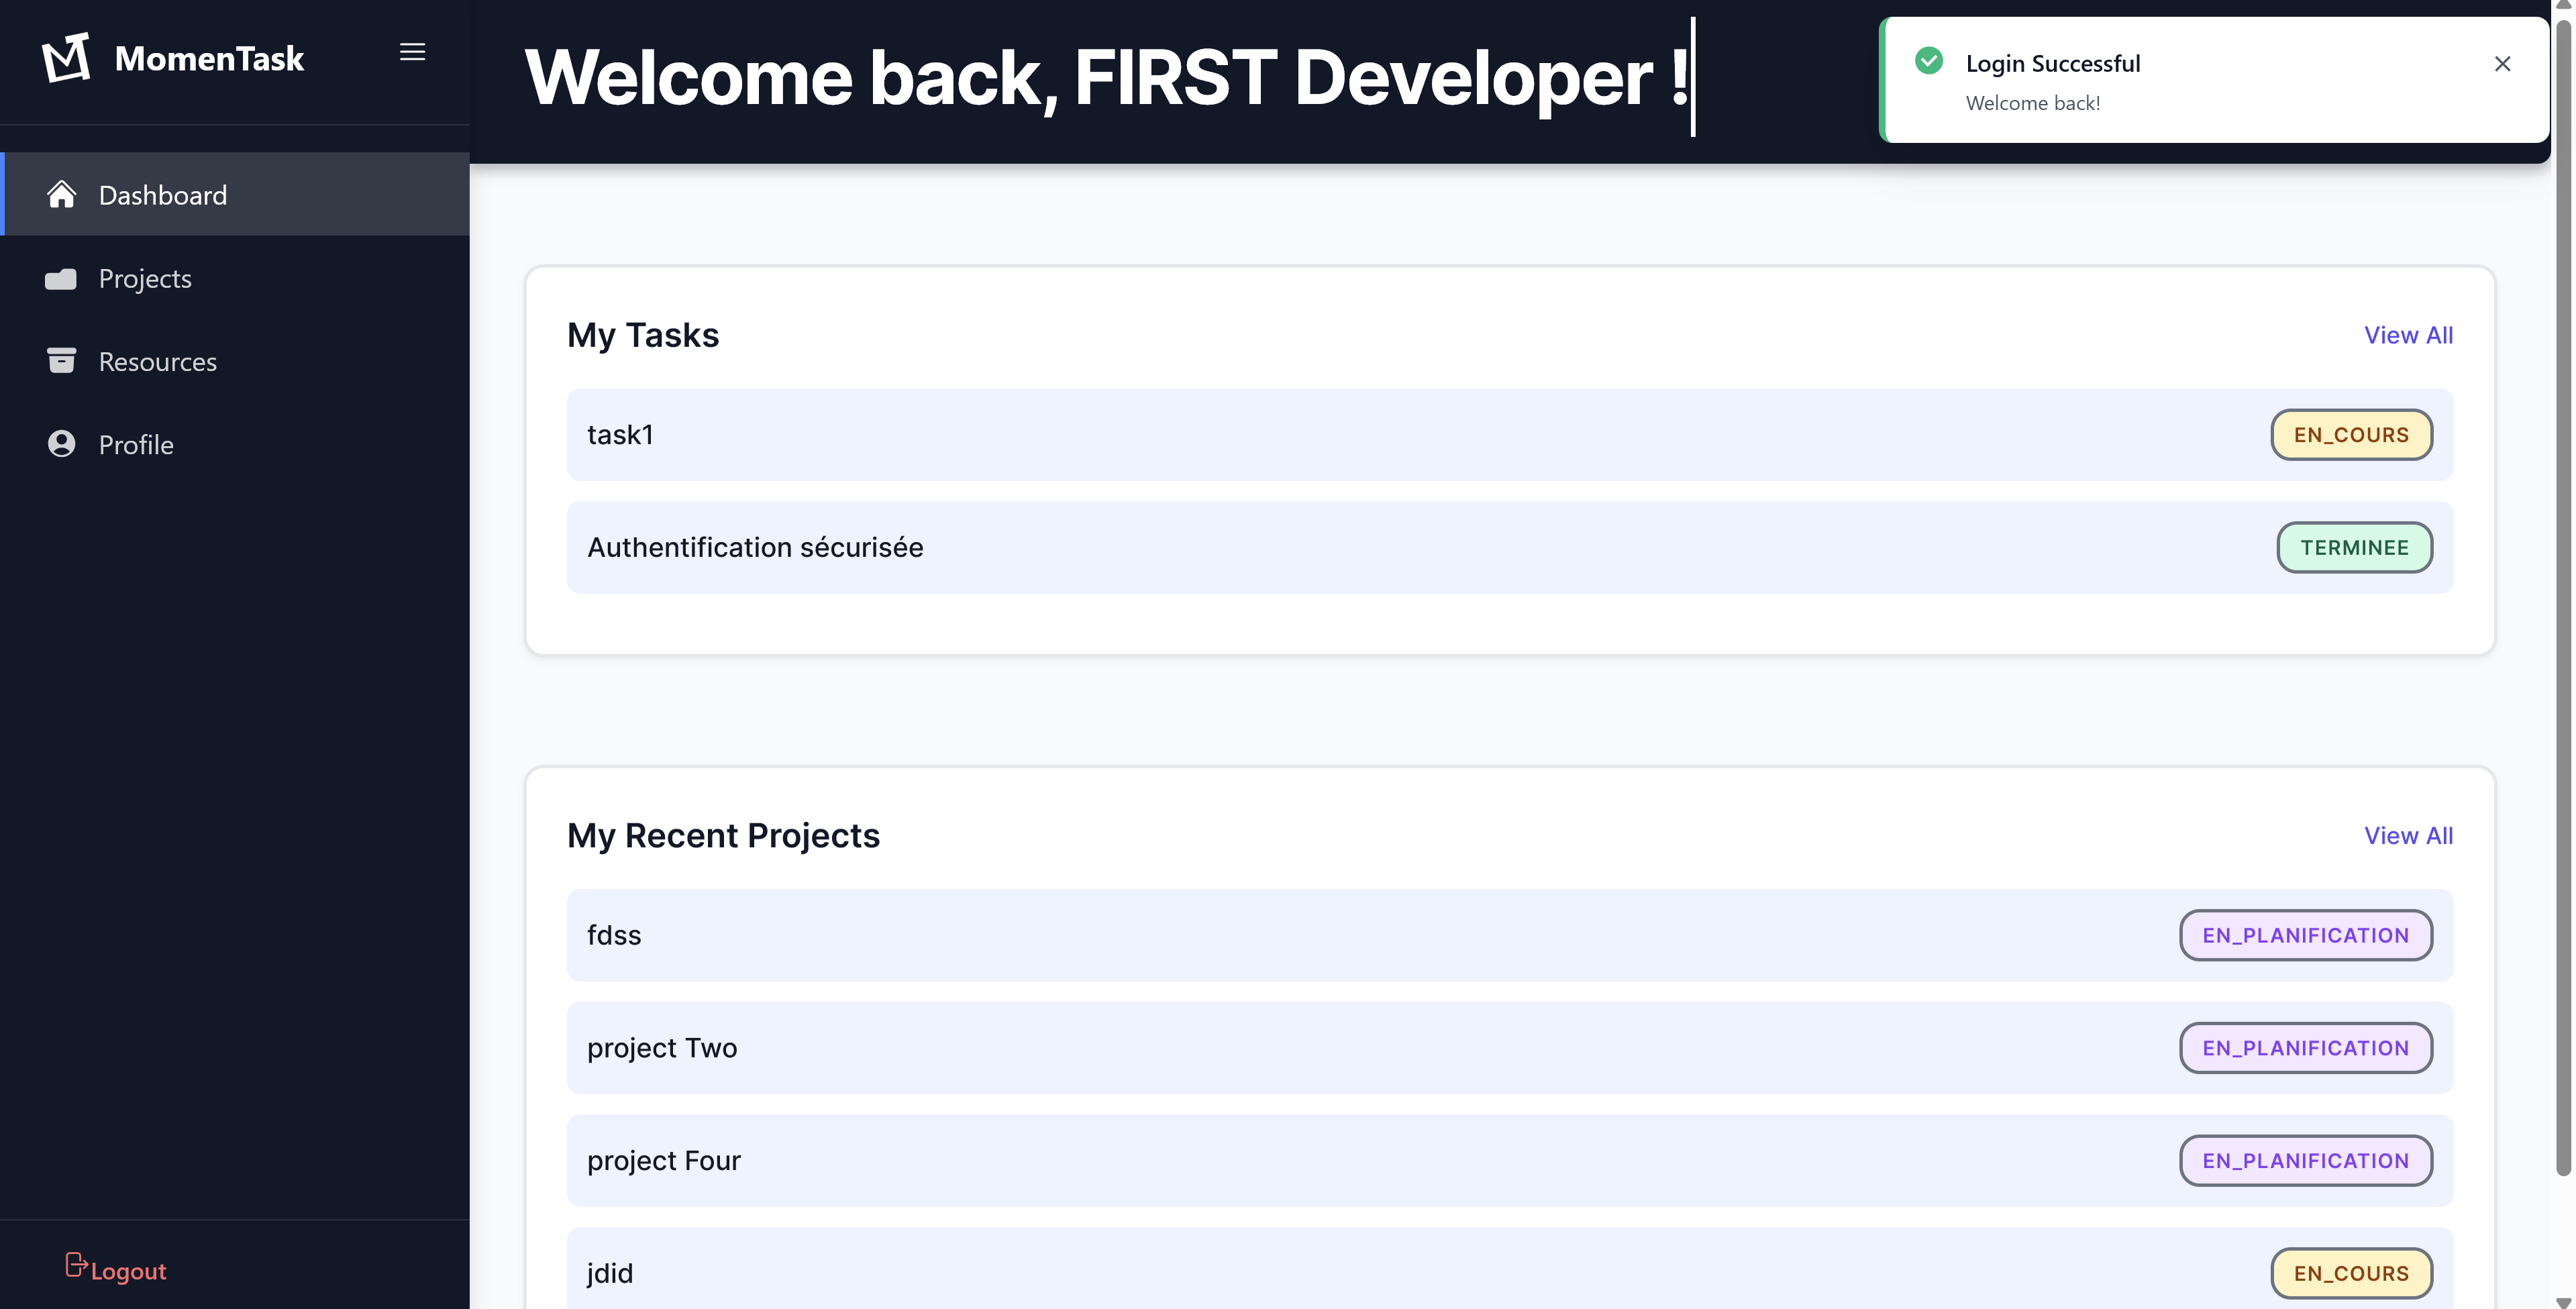
\includegraphics[width=\textwidth]{Figures/pm screenshots/dev/dashboard.png}
    \caption{Tableau de bord développeur avec tâches et projets récents}
    \label{fig:dev-dashboard}
\end{figure}

Ce tableau de bord personnalisé pour les développeurs présente leurs tâches assignées et leurs projets récents. Il affiche les tâches avec leurs statuts (EN\_COURS, TERMINEE) et les projets avec leurs phases (EN\_PLANIFICATION, EN\_COURS). L'interface offre une vue d'ensemble rapide du travail en cours et des priorités.

% --- Interface Assigned Tasks ---
\begin{figure}[H]
    \centering
    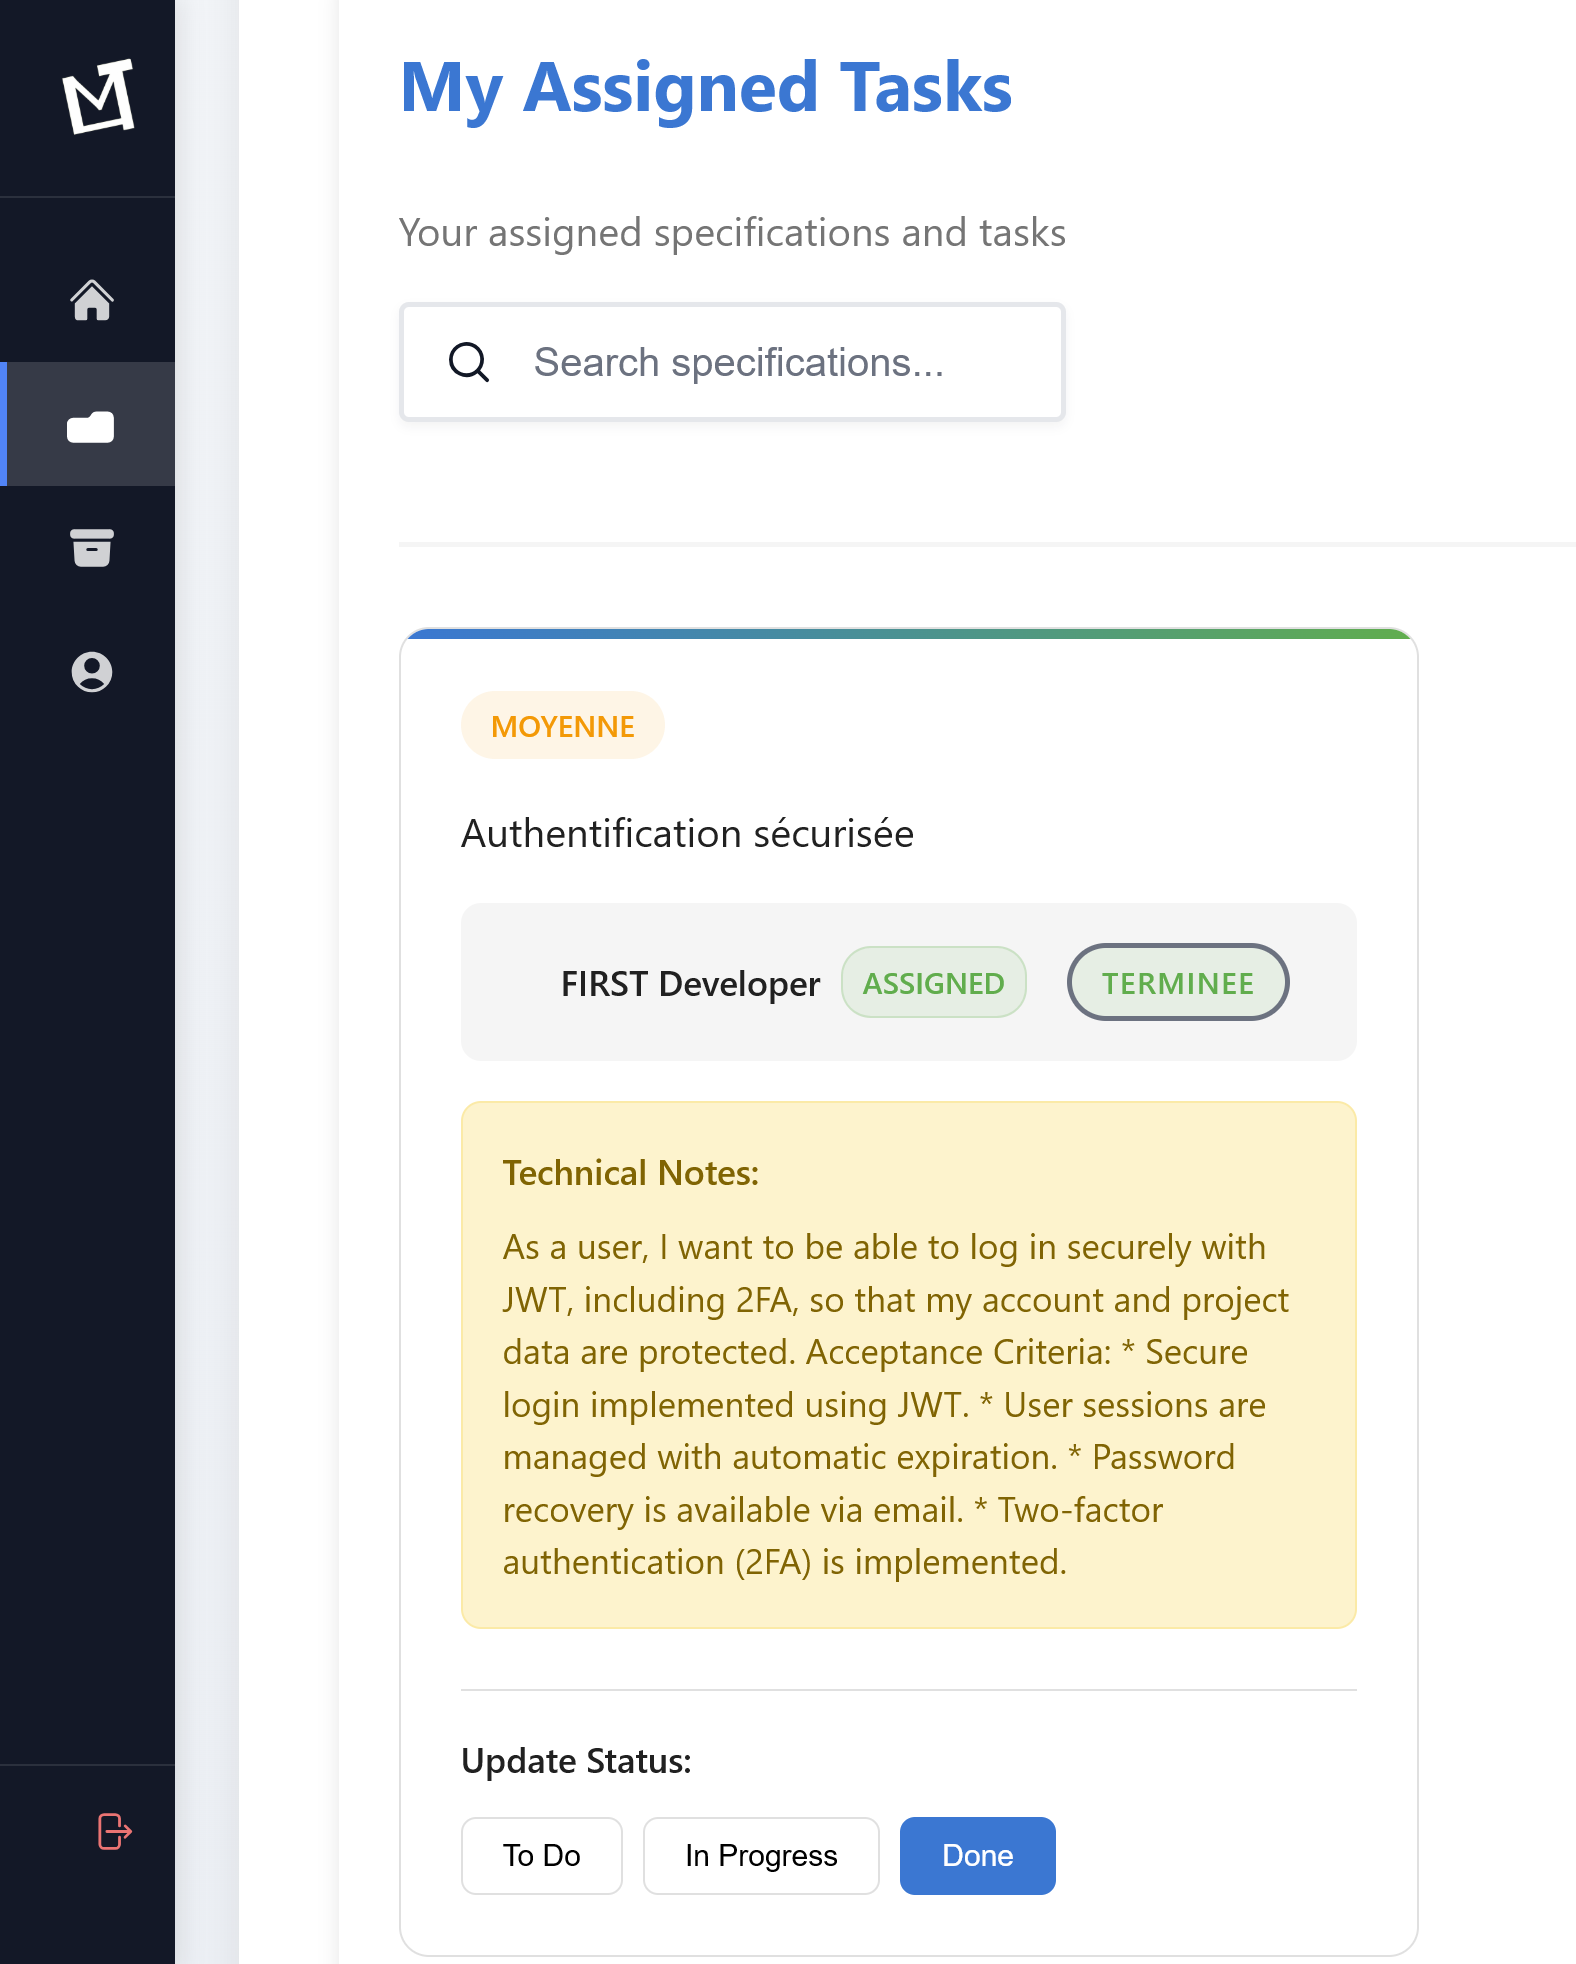
\includegraphics[width=\textwidth]{Figures/pm screenshots/dev/ITERATIF assigned tasks.png}
    \caption{Interface des tâches assignées avec détails techniques}
    \label{fig:dev-assigned-tasks}
\end{figure}

Cette interface présente les tâches assignées au développeur avec tous les détails techniques nécessaires. Elle affiche les spécifications, critères d'acceptation, et permet la mise à jour du statut des tâches (To Do, In Progress, Done). L'exemple montre une tâche d'authentification sécurisée avec JWT et 2FA.

% --- Interface Kanban Board ---
\begin{figure}[H]
    \centering
    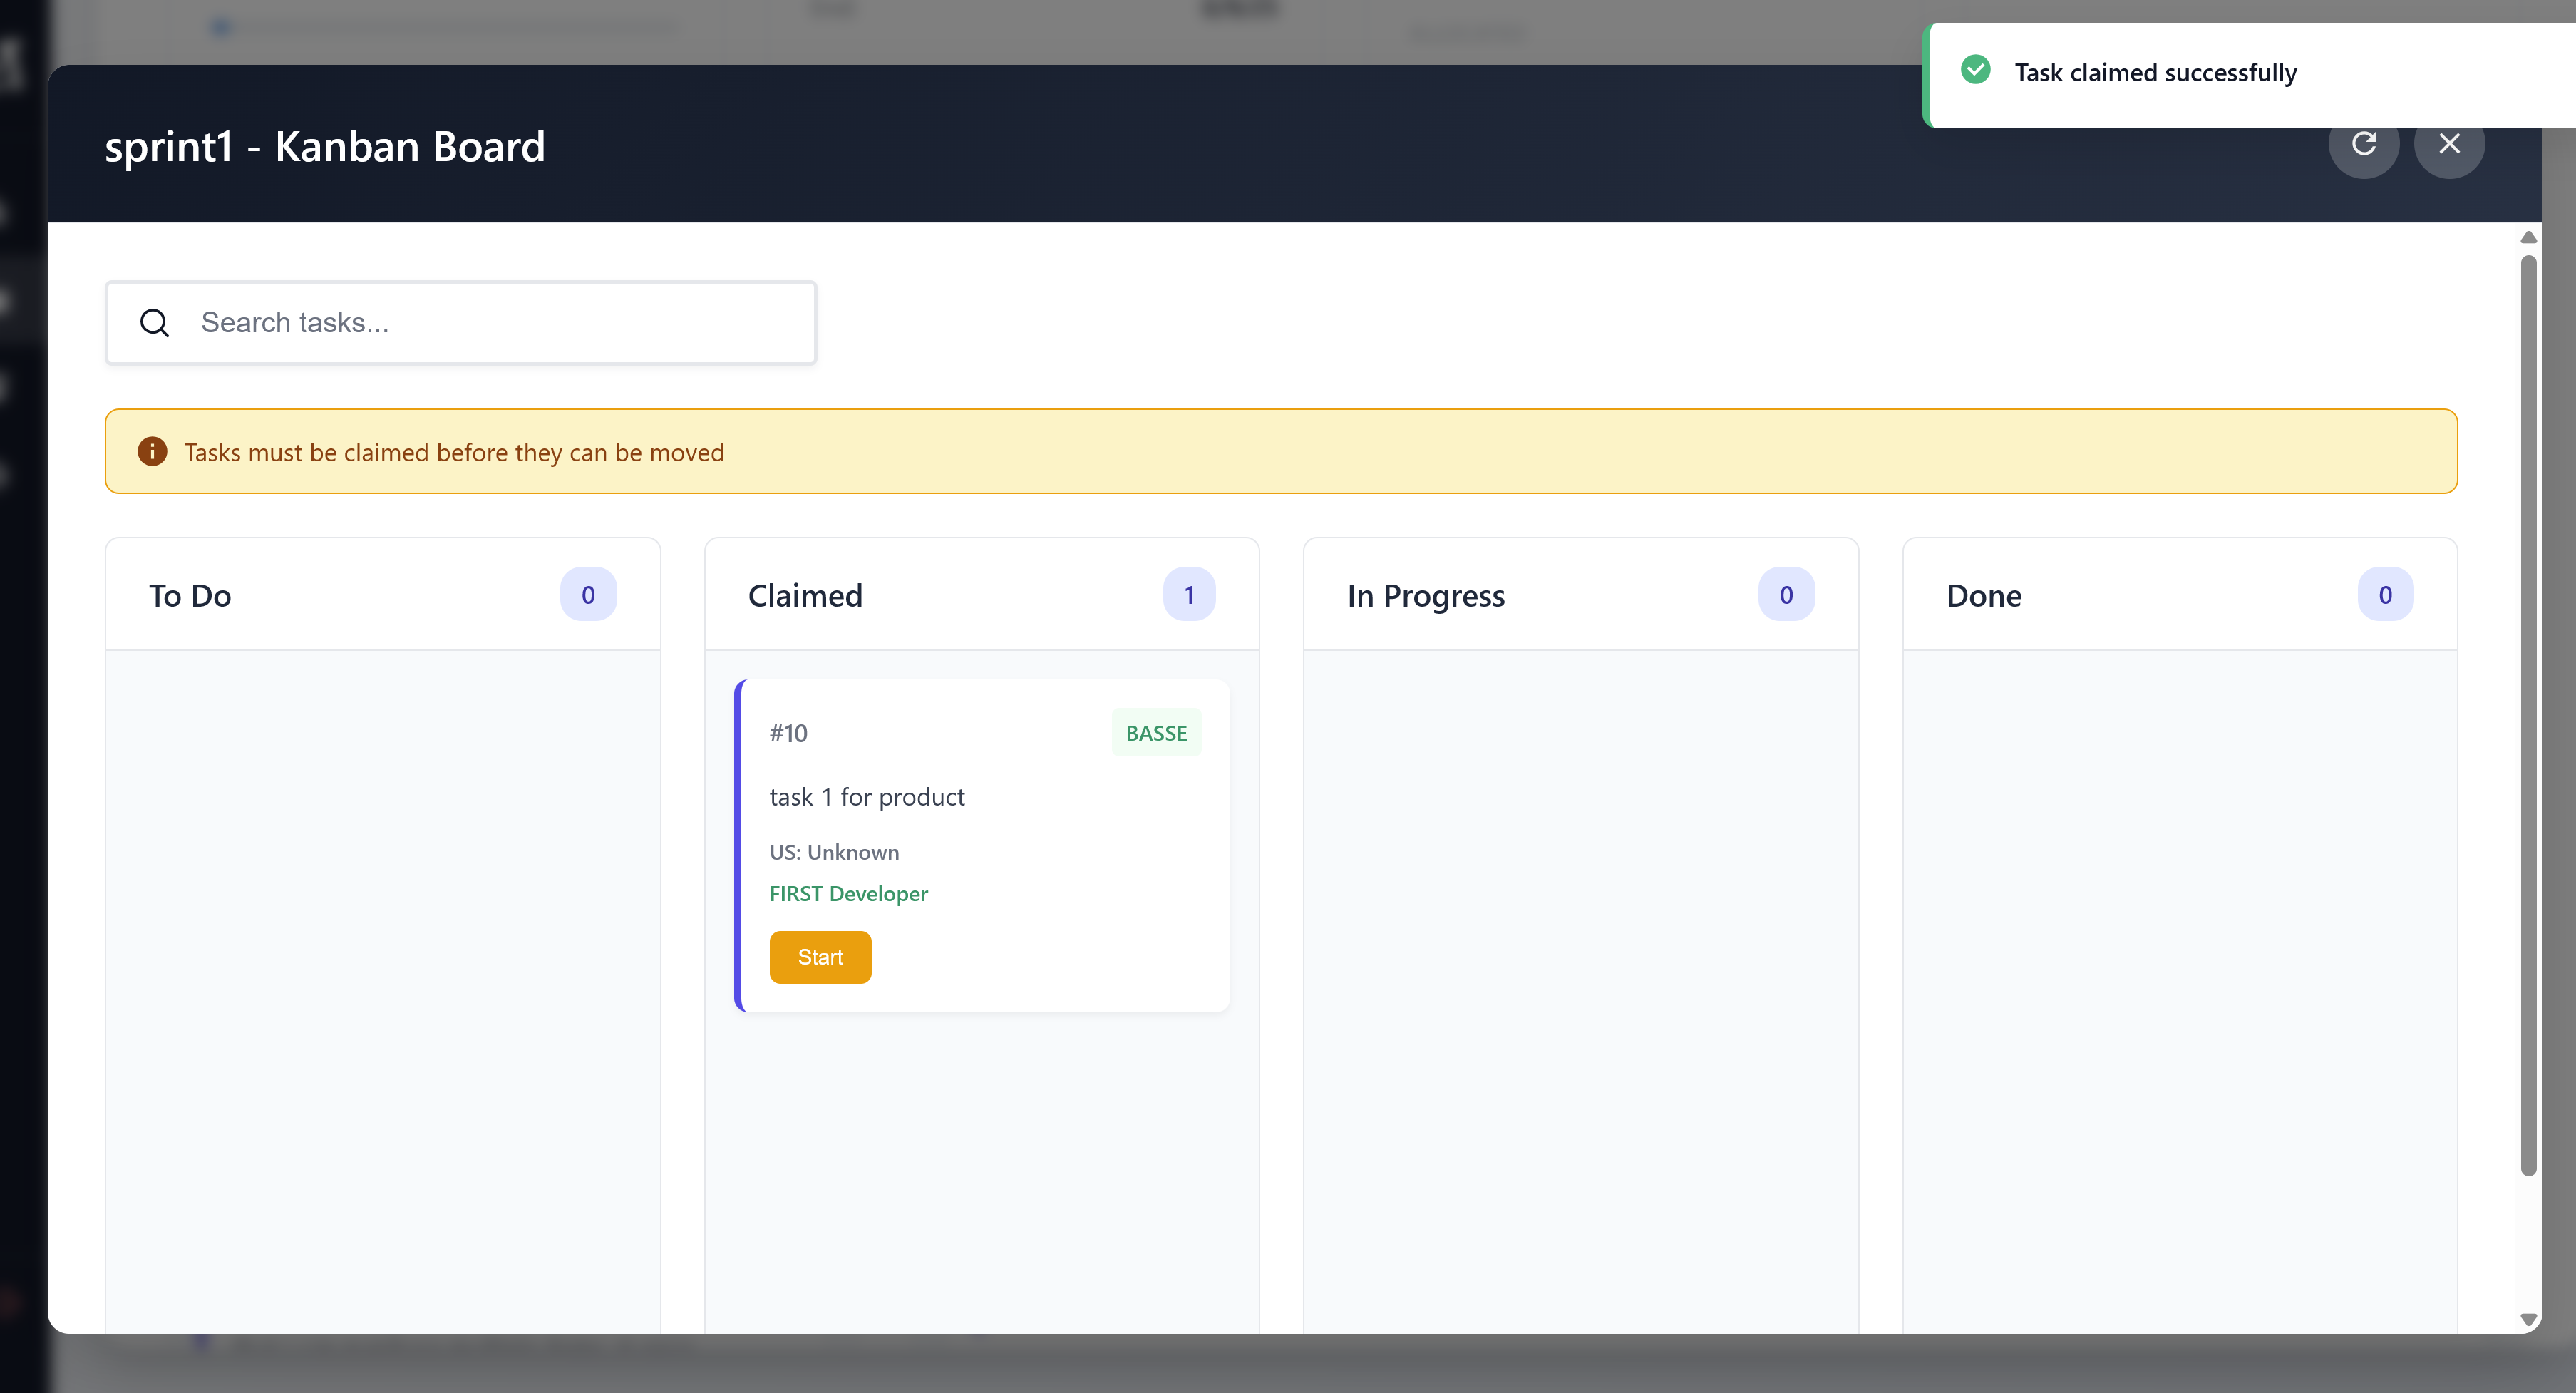
\includegraphics[width=\textwidth]{Figures/pm screenshots/dev/kanban board.png}
    \caption{Tableau Kanban pour la gestion des tâches de sprint}
    \label{fig:dev-kanban}
\end{figure}

Cette interface Kanban permet aux développeurs de visualiser et gérer les tâches du sprint. Elle organise les tâches en colonnes (To Do, Claimed, In Progress, Done) et affiche les détails de chaque tâche (ID, priorité, description, assignation). L'interface facilite le suivi du flux de travail et la collaboration en équipe.

% --- Interface Sprints ---
\begin{figure}[H]
    \centering
    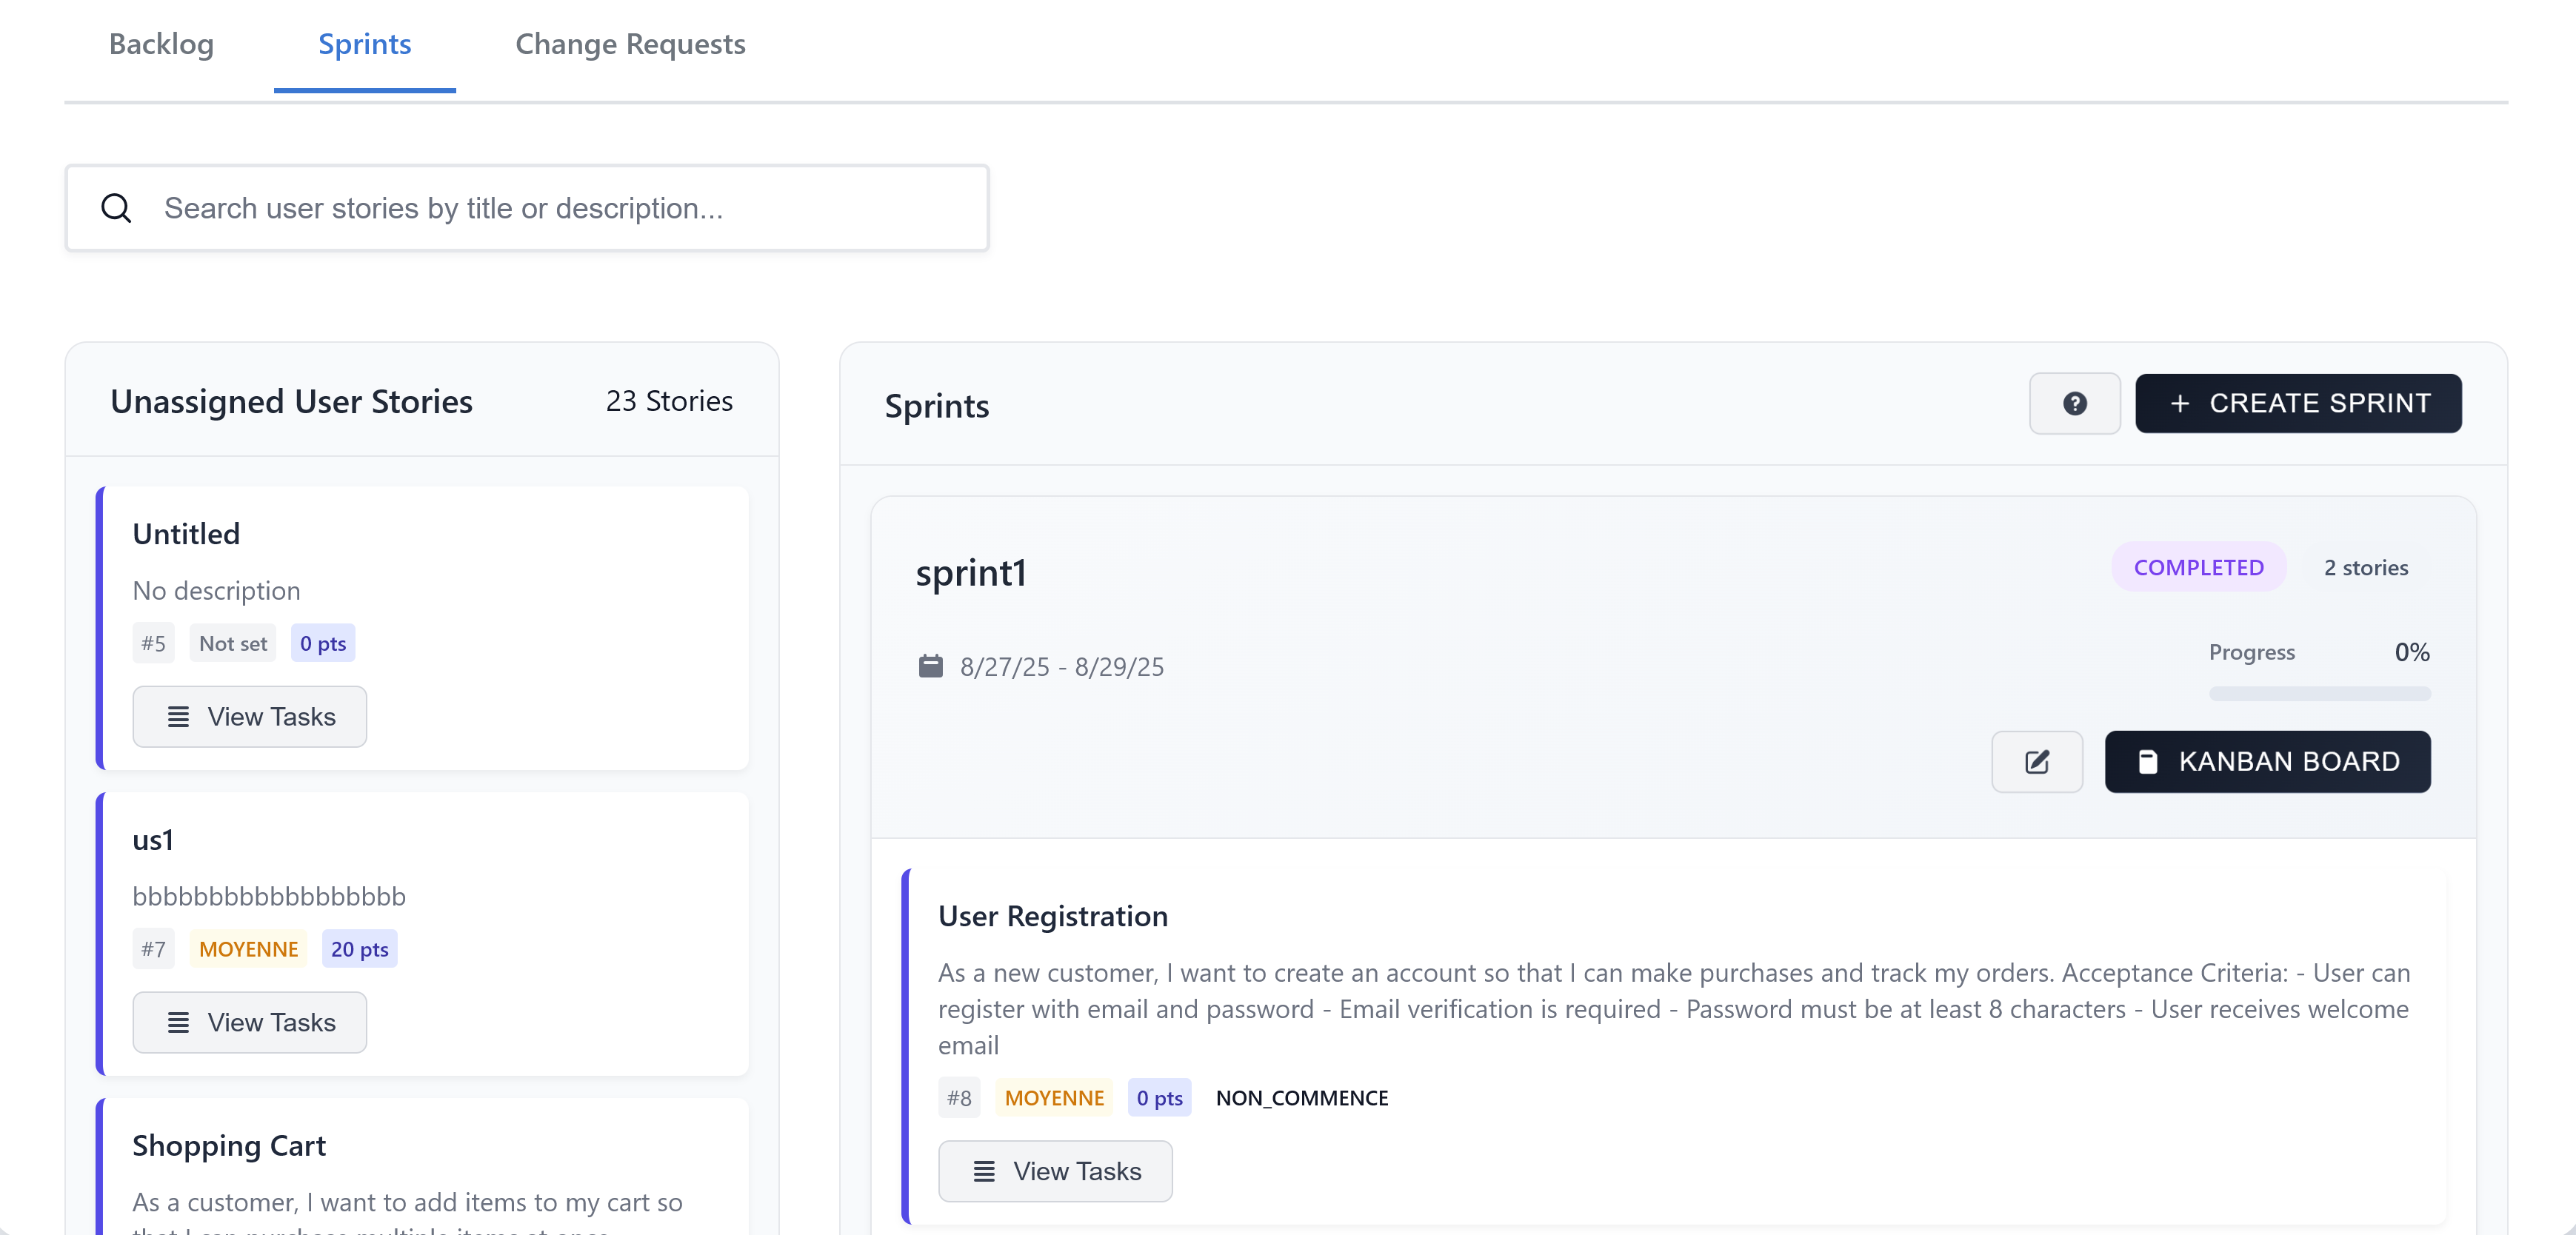
\includegraphics[width=\textwidth]{Figures/pm screenshots/dev/sprints.png}
    \caption{Interface de gestion des sprints et user stories}
    \label{fig:dev-sprints}
\end{figure}

Cette interface permet de gérer les sprints et d'organiser les user stories. Elle présente les user stories non assignées et les sprints existants avec leurs détails (dates, statut, progression). L'interface facilite la planification des sprints et l'assignation des user stories aux différentes itérations.

\subsection{Vue Itératif}

% --- Interface Milestones ---
\begin{figure}[H]
    \centering
    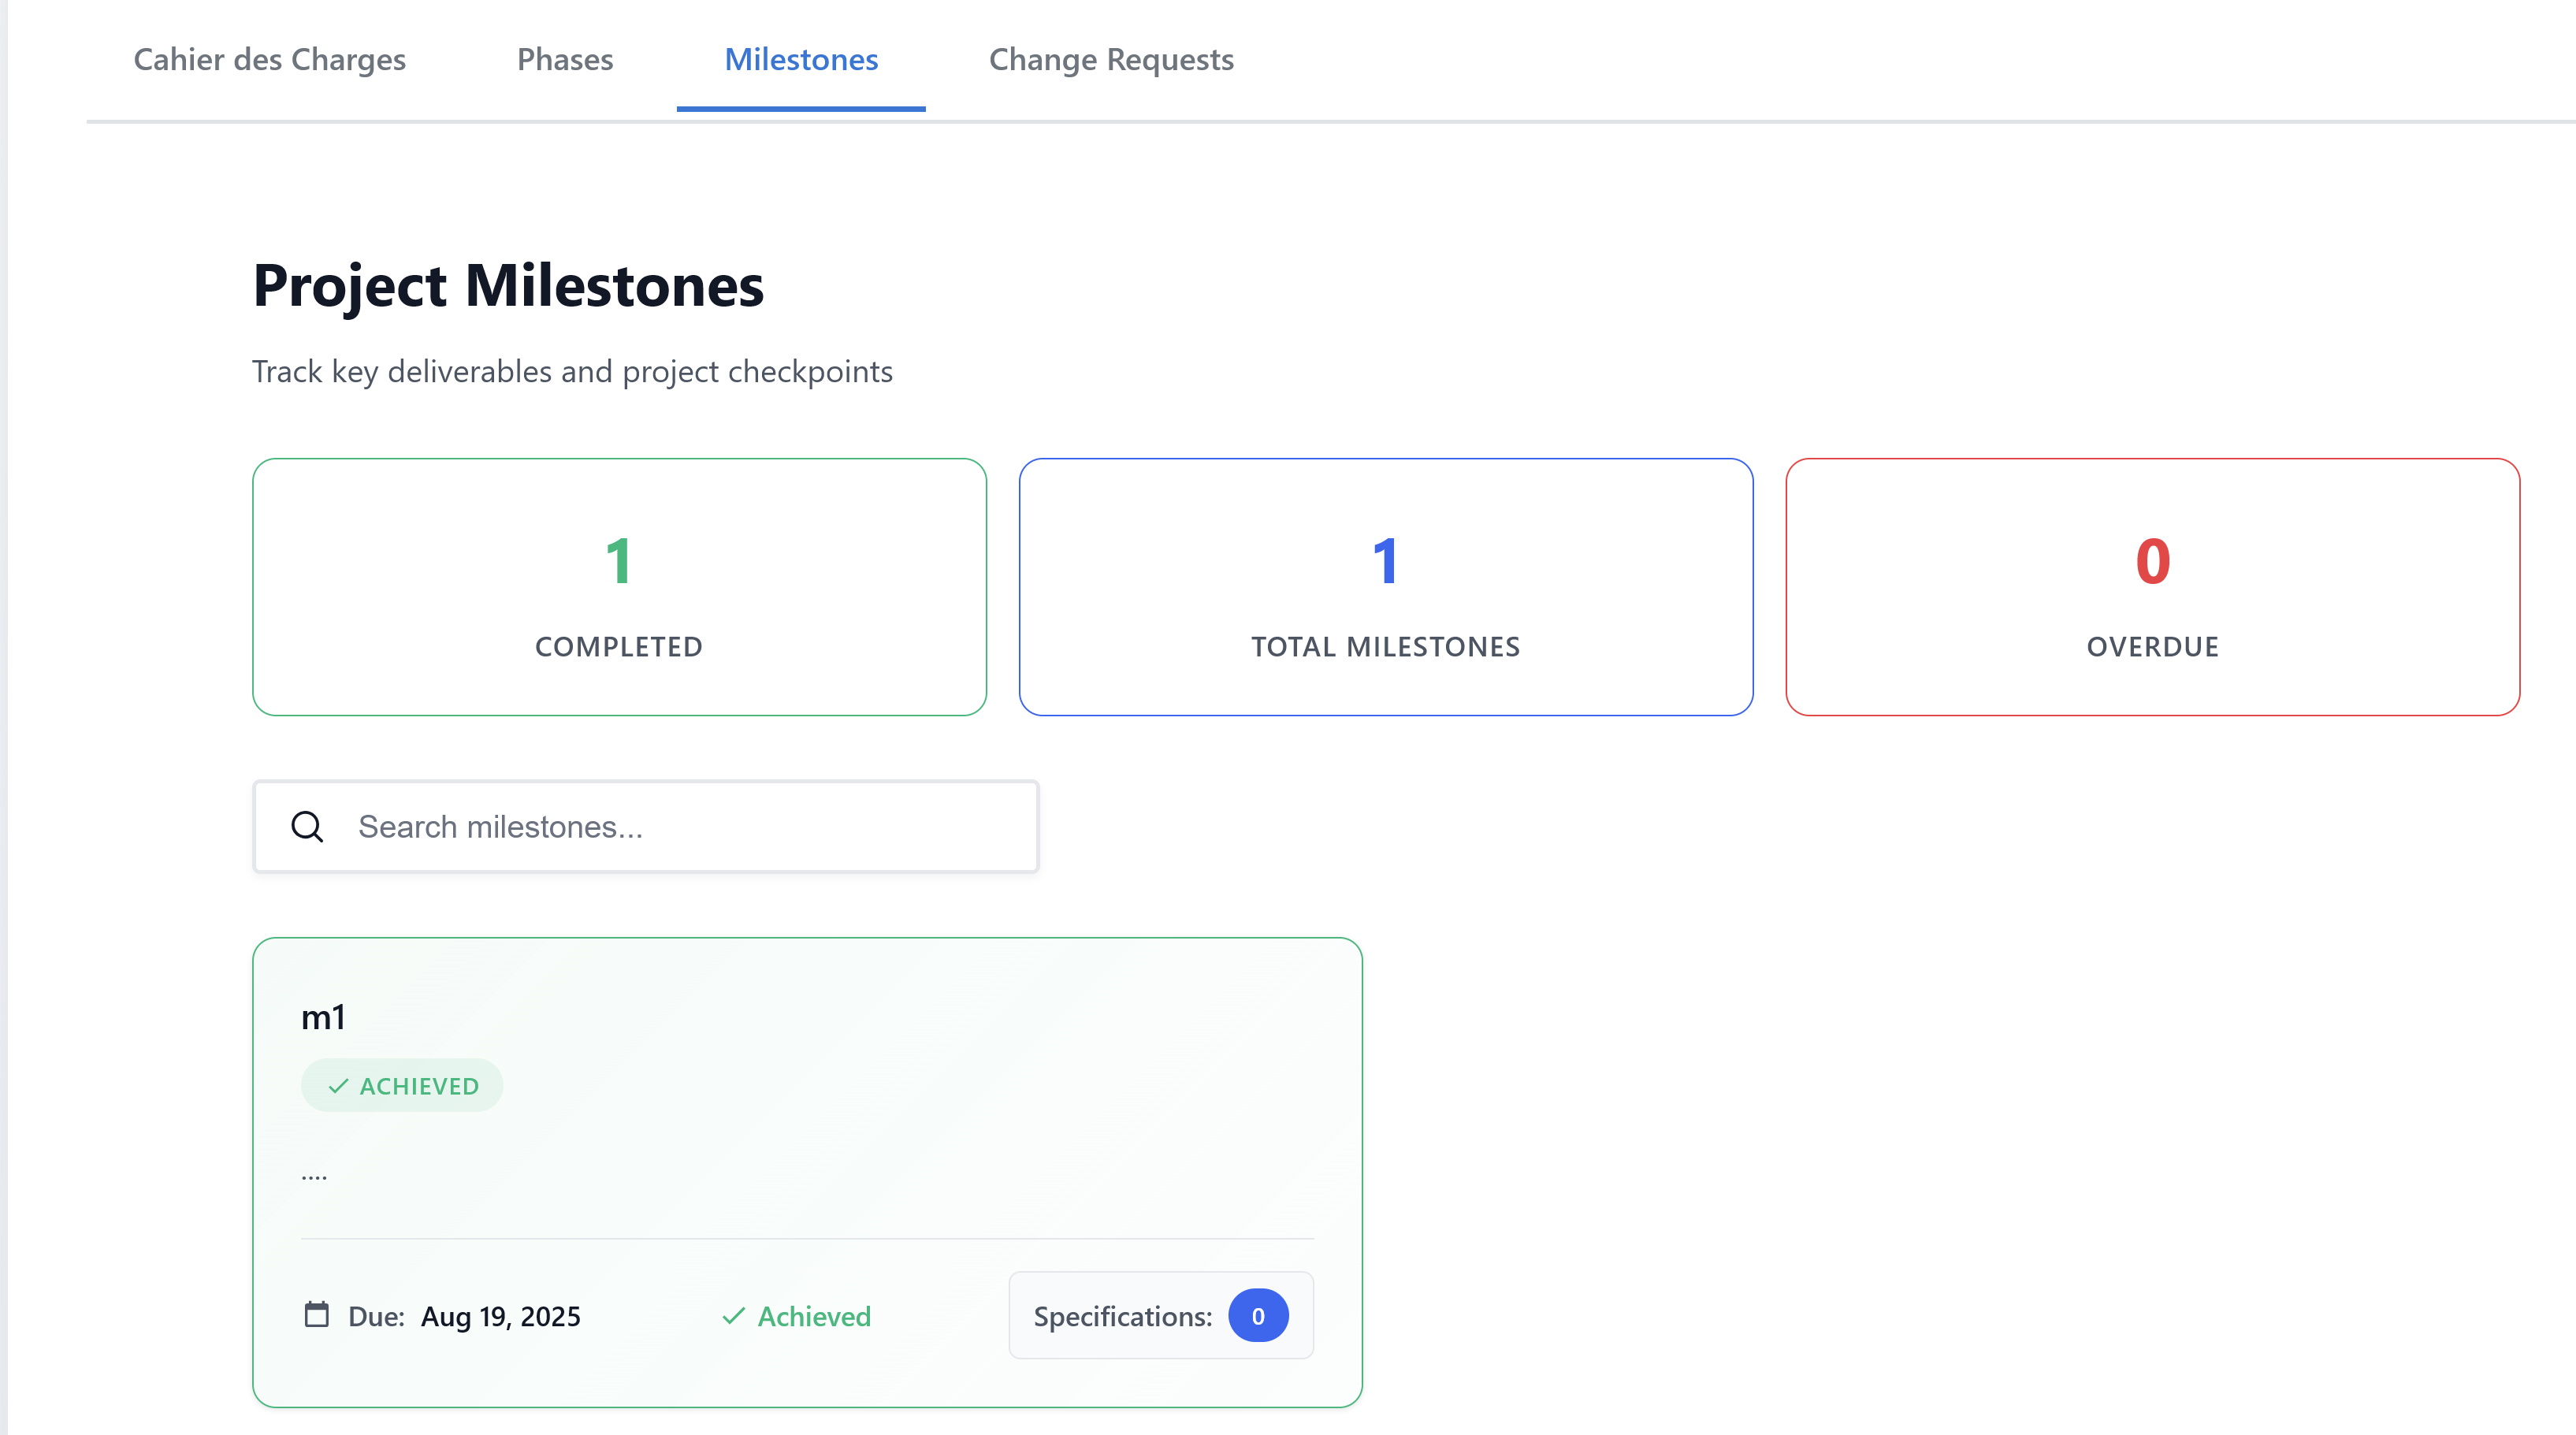
\includegraphics[width=\textwidth]{Figures/pm screenshots/iteratif milestones.png}
    \caption{Interface de gestion des jalons de projet}
    \label{fig:iteratif-milestones}
\end{figure}

Cette interface permet de gérer les jalons (milestones) du projet dans une approche itérative. Elle affiche les jalons avec leurs statuts (ACHIEVED), dates d'échéance, et livrables associés. L'interface propose des métriques de suivi (complétés, total, en retard) et facilite la planification des phases du projet.

% --- CONCLUSION DU CHAPITRE ---
\section{Conclusion}
En somme, ce chapitre a présenté l’architecture microservices et les technologies choisies pour développer une application à la fois performante, fiable et évolutive.
Les interfaces conçues offrent une expérience utilisateur fluide et intuitive, tout en facilitant la gestion centralisée des services.
La prise en charge du multilinguisme et l’intégration de statistiques renforcent la flexibilité et la valeur décisionnelle de la solution.